%%
%% Meta: Formelsammlung GESO BBW
%% 2021 fp @ bbw.ch
%%

%% Footer und Header ganz unterdrücken:
\newcommand{\keinHeaderUndKeinFooter}{}
%% Sollten Header und Footer unterdrückt werden, einfach die folgende
%% Zeile nicht als Kommentar lassen:
%%\renewcommand{\keinHeaderUndKeinFooter}{\thispagestyle{empty}}


\newcommand{\versionsDatumFoSa}{2021-11-29}

%% ID (ca. alle jahre), Subversion: Grössere Änderungen, Revision: Jede
%% Umstellung/Korrektur/Typos
\newcommand{\versionIdSubRev}{0.4.0}


%% ID (ca. alle jahre), Subversion: Grössere Änderungen, Revision: Jede
%% Umstellung/Korrektur/Typos

\newcommand{\versionsnummerFoSa}{\versionsDatumFoSa{} \versionIdSubRev}

%% Für Notationen   mit a, b, c (Hersberger Christian [HECH])
%% Für Schreibwesie mit m, q etc. (Rahmenlehrplan [RLP])
\newif\ifisHECH
\newif\ifisRLP

%% Steuere später über das File "VERSION.sty"
%%\isHECHtrue %% f(x) = ax+b
%%\isRLPtrue %%f(x) = mx+q
%%
%% Steuerung, ob die Variablennamen nach RLP (Rahmenlehrplan) oder
%% nach Ch. Hersberger (HECH) verwendet werden sollten. 

\isRLPtrue
%%\isHECHtrue


%% Kommandos zur Vereinfachun des Einbindens der beiden Versionen
\newcommand\HECH[1]{%%
{%%
\ifisHECH{#1}%%
\fi%%
}}%% End New Command HECH
%% Für Rahmenlehrplan (RLP)
\newcommand\RLP[1]{%%
{%%
\ifisRLP{#1}%%
\fi%%
}}%% End New Command RLP

%% Philipp G Freimann Juli 2019 für die BBW
%% Phi BBW-Vorlage für Arbeitsblätter (LaTeX)
%% 2019 - 08 - 18

%% %% %% %%


%%  In den Dokumenten können die folgenden Attribute überschrieben werden:


\newcommand{\metaHeaderLine}{HeaderLine mit $\backslash{}$ metaHeaderLine überschreiben}

%% \thema
\newcommand{\arbeitsblattTitel}{Pruefungsthema mit renewcommand
  arbeitsblattTitel überschreiben.}


%%%%%%%%%%%%%%%%%%%%%%% P A C K A G E S %%%%%%%%%%%%%%%%%%%%%%%%%%%%%
\usepackage[paper=a4paper,margin=17mm]{geometry}

%%\usepackage{german} %% Macht Probleme mit grafiken
\usepackage{mciteplus}

\usepackage[dvipsnames]{xcolor}

\usepackage{pgfplotstable}
\usepackage{tikz}
\usepackage{tkz-euclide} %% Grid

\usepackage{amsthm}
\usepackage{amsfonts} %% Zahlmengen Z, R, ...


%% THEOREMS?
\usepackage{tcolorbox}
\tcbuselibrary{theorems}
\tcbuselibrary{skins}


\usepackage{fancyhdr}
\usepackage{ngerman}
\usepackage[utf8]{inputenc}


%%\usepackage[dvips]{graphicx}

\usepackage{supertabular}
\usepackage{makeidx}  
\usepackage{ifthen} 

\usepackage{multirow}
\usepackage{listings}

%%\usepackage{color,fancyvrb,fancybox}
\usepackage{multicol}
\usepackage{lastpage}
%%\usepackage{listings}
\usepackage{pstricks}

%% bold typewriter font:
\usepackage[T1]{fontenc}
\usepackage{lmodern}

\usepackage{enumitem}
%\usepackage{enumerate}

\usepackage{float}

\usepackage{titlesec}
\usepackage{textcomp}

%% Kuchendiagramme
%%\usepackage{datapie}

%% für Aufgaben Hervorhebung
%%\usepackage[most]{tcolorbox}
%%\usepackage[standard,framed]{ntheorem}
\usepackage{framed}
\usepackage{mdframed}

%%%%%%%%%%%%%%%%%%%%
%%\usepackage[most]{tcolorbox}

\usepackage[tocindentauto]{tocstyle}

%% für accentset wedge:
\usepackage{accents}

%% Würfel
\usepackage{epsdice}

%% Einbinden von GeoGebra Bildchen:
\usetikzlibrary{shapes.geometric}
\usetikzlibrary{arrows}
\newcommand{\degre}{\ensuremath{^\circ}}

%% Hyperlinks
\usepackage{hyperref}

\hypersetup{
    colorlinks=true,
    linkcolor=blue,
    filecolor=magenta,      
    urlcolor=cyan,
    bookmarks=true,
}

%% bugtracker (part of pgfplots) should be loaded AFTER "hyperref"
%% See: https://texblog.net/hyperref/ AND https://tex.stackexchange.com/questions/16268/warning-with-footnotes-namehfootnote-xx-has-been-referenced-but-does-not-exi
\usepackage{pgfplots}
\pgfplotsset{width=10cm,compat=1.9}


\usepackage{tgheros}%% Font TeX Gyre Heros für Titel (font code qhv)

%% damit die Punktezal schon geschrieben werden kann, obschon
%% Die Punkte erst während dem Dokument zusammengetragen werden:

%%%%%%%%%%%%%%% L A Y O U T  %%%%%%%%%%%%%%%%%%%%%%%%%%%%
%% 2020-12-27 ph. g. freimann @ bbw.ch
%%

\fancyhf{}%%

\pagestyle{fancy}%%

\renewcommand{\sectionmark}[1]{%%
  \markboth{\thesection{} \ #1}{}%%
}%%

\renewcommand{\subsectionmark}[1]{%%
  \markright{\thesubsection \ #1}%%
}%%

%% Achtung: chaptermark nur im BOOK-Style

\renewcommand{\footrulewidth}{0.4pt}

\parskip4pt
\parindent0pt

\topmargin-2.0cm
\textheight24.4cm

\renewcommand{\arraystretch}{1}%%

%%%%%%%%%%%%%%%%%%%%%%%%%%%%%%%%%%%%%%%%%%%%%%%%%%%%%%%%%%
%%%%%%%%%%%%%%%%%% M A K R O S %%%%%%%%%%%%%%%%%%%%%%%%%%%
%%%%%%%%%%%%%%%%%%%%%%%%%%%%%%%%%%%%%%%%%%%%%%%%%%%%%%%%%%

%%%%%%%%%%%%%%%%%%%%%%%% g e n e r e l l e   M a k r o s %%%%%%%%%%%%%%%%%%%%%%%

%% 2019-07-26
%% phi@freimann.eu
%% Makros for BBW-Tex Documents
\usepackage{inputs/bbwColors}

%%%%%%%%%%%%%%%%%% I N C L U D E S   &   I N D E X  %%%%%
\graphicspath{{../img/}}
\graphicspath{{./img/}}

\newcommand\bbwGraphicRaise[3]{\raisebox{#1}{\includegraphics[width=#2]{#3}}}%%
\newcommand\bbwGraphic[2]{\bbwGraphicRaise{-5mm}{#1}{#2}}%%
\newcommand\bbwCenterGraphicRaise[3]{\begin{center}\bbwGraphicRaise{#1}{#2}{#3}\end{center}}
\newcommand\bbwCenterGraphic[2]{\bbwCenterGraphicRaise{-5mm}{#1}{#2}}%%


%% All in one Skript
\newif\ifisALLINONE
\isALLINONEfalse

%%%%%%%%% TRAINER Version vs. Schülerversion %%%%%%%%%%%%%

\newcommand\TRAINER[1]{%%
{%%
\ifisTRAINER{\color{BlueGreen}{#1}}%%
\fi%%
}}%%  

\newcommand\TALS[1]{%
{%%
\ifisTALS {#1}%%
\fi%%
}}%

\newcommand\GESO[1]{%
{%%
\ifisGESO {#1}%%
\fi%%
}}%    

\newcommand{\noTRAINER}[1]{{\ifisTRAINER{}\else{#1}\fi}{}}%%



%%\makeatletter
%% Je nach Umgebung "environment" wird das mmPapier breiter oder
%% schmaler
%% bei itemize sollen 16.4 und bei definiton-Boxen 16.8 mm genommen
%% werden.


\usepackage{inputs/mmPapierbreiteSty}


%% Trainer "no" Dotfill
%% If no Trainer: Dotfill
\newcommand{\TNDF}[1]{\TRAINER{#1}\noTRAINER{\dotfill{}}}%%

\newcommand{\leserluft}{\vspace{2mm}}

%% Notiz felder 
%% Anwendung:
%% \noteField{10}  
%%  --> Notizfeld mit 10 Leerzeilen
\newcounter{DFCounter}

\newcommand*{\noteField}[1]{%
\setcounter{DFCounter}{1}
\vspace{0.5in}%
\begin{tabular}{p{14cm}}%
\hline%
\vspace{0.2cm}
Notizen: \\%
\whiledo{\theDFCounter < #1}{%
\dotfill \\
\addtocounter{DFCounter}{1}%
}%
\end{tabular}%
}%

\newcommand*{\noteLines}[1]{%
\setcounter{DFCounter}{1}
\vspace{0.1cm}%
\begin{tabular}{p{14cm}}%
\whiledo{\theDFCounter < #1}{%
\dotfill \\
\addtocounter{DFCounter}{1}%
}%
\end{tabular}%
}%

%% Platz für Notizen, aber nur bei Schülernverison (\noTRAINER)
\newcommand{\platzFuerTNNotes}[1]{%
\ifisTRAINER{}\else{%%
Platz für Notizen:\newline%%
\noteLines{#1}%%
}\fi{}%
}%%

%% Vier Leerzeilen für Notizen
\newcommand*\dotfillpara{%
\begin{tabular}{p{11.5cm}}%
\hfill   \\
\dotfill \\
\dotfill \\
\dotfill \\
\dotfill
\end{tabular}%
}


%%Häuschenpapier
\newcommand{\mmPapierZwei}[2]{\begin{tikzpicture}
%%  \draw[step=4mm,bbwMMFarbe,ultra thin]
%%  \draw[step=4mm,bbwMMFarbe,thick]
  \draw[step=4mm,bbwMMFarbe,line width=0.02mm]
  (0, 0) grid ({#2}, {#1});
\end{tikzpicture}}%%


%% millimeterPapier füllen bis Ende Seite
\newcommand{\mmPapierBisEndeSeite}{

\begin{tikzpicture}

\newdimen\spaceleftOnPage
\spaceleftOnPage=\dimexpr\textheight-\pagetotal-14pt\relax

\pgfmathsetmacro{\gridWidth}{\textwidth        - mod(\textwidth,      4mm)      }
\pgfmathsetmacro{\gridHeight}{\spaceleftOnPage - mod(\spaceleftOnPage,4mm) - 4mm}

\draw [step=4mm,bbwMMFarbe,line width=0.02mm] (0,0) grid (\gridWidth pt,\gridHeight pt);
\end{tikzpicture}%%
\newpage%%
}%% END Makro mmPapieBisEndeSeite


%% Standardbreite für Arbeitsblätter und das Theorieheft
%% Wird in bbwPruefung.sty überschrieben, da dort schmaler
\def\defaultTextBreite{17.6}
\def\unitCMWhatElse{cm}%% wird als Breitenangabe für den nächsten command verwendet

%% Verwendung: \bbwCenterGraphic{\defaultTextBreite}{«img url»}
\def\defaultTextBreiteCM{\defaultTextBreite\unitCMWhatElse}
\newcommand{\mmPapier}[1]{\mmPapierZwei{#1}{\defaultTextBreite}}


%% Notizen Berechungen auf Prüfungsblättern
\newcommand{\platzFuerBerechnungen}[1]{\noTRAINER{

Notizen / Berechnungen:

\mmPapier{#1}}}%% end platzFuerBerechnungen

\newcommand{\platzFuerBerechnungenBisEndeSeite}[1]{\noTRAINER{

Notizen / Berechnungen:

\mmPapierBisEndeSeite}}%% end platzFuerBerechnungen



\newcommand{\platzFuerBerechnungenOhneText}[1]{\noTRAINER{

\mmPapier{#1}}}


%% Die Abkürzung z.\,B. von «Zum Beispiel» hat einen verkleinerten Abstand.
\newcommand*\zB{%
z.\,B.
}

%%
%% Auf der Titelseite steht entweder GESO oder TALS.
%% Dies wird gleich mit der Fußnote angegeben.
%% Dieses Kommando sollte im Kommando «\untertitel» eingesetzt werden.
%%
\newcommand*\ausrichtungAufTitelseite{%
\ifisTALS{TALS\noTRAINER{\footnote{TALS «Technik, Architektur und Life Sciences
(Laboranten)»: Ausrichtung technisches Profil}}}%%
\fi%%
\ifisGESO{GESO\noTRAINER{\footnote{GESO: Ausrichtung \textbf{Ge}sundheit und \textbf{So}ziales}}}%%
\fi}%%

%%%%%%%%%%%%%%%%%%%%%% B B W - M a t h e   F a r b c o d e s  %%%%%%%%%%%%%%%%%%%%%%%%%%%%%%555

\newcommand{\rezeptFarbe}{rezeptFarbe}
\newcommand{\definitionFarbe}{definitionFarbe}
\newcommand{\gesetzFarbe}{gesetzFarbe}
\newcommand{\beispielFarbe}{beispielFarbe}
\newcommand{\bemerkungFarbe}{bemerkungFarbe}

%% Falls gewünscht übersteuren
%  \definecolor{xyz}{HTML}{eeff66}
%  \renewcommand{\beispielFarbe}{xyz}
%

%% Theorem-Styles
\newcommand\theoremlayoutdefinition[4]{\newtcbtheorem[number within=section]{#1}{#2}%
   {theorem style=plain,enhanced,colframe=#3!20!white,colback=#3!20!white,
     coltitle=#3!60!black,fonttitle=\upshape\bfseries,
     %%fontupper=\itshape,
    %%drop fuzzy shadow=blue!50!black!50!white,
    terminator sign={:},
    borderline north={0.5mm}{0pt}{#3}, borderline south={0.5mm}{0pt}{#3}
   }{#4}}



%% Farben für rezept, definition und gesetz von Marthale übernommen.
%% Verwendung mit * unterbindet die Nummerierung \begin{gesetz*}{Blah}{xy} ...\end {gesetz*}
\theoremlayoutdefinition{rezept}{Rezept}{\rezeptFarbe}{R}
\theoremlayoutdefinition{definition}{Definition}{\definitionFarbe}{D}
\theoremlayoutdefinition{gesetz}{Gesetz}{\gesetzFarbe}{G}%% was green
\theoremlayoutdefinition{beispiel}{Beispiel}{\beispielFarbe}{B}
\theoremlayoutdefinition{bemerkung}{Bemerkung}{\bemerkungFarbe}{M}


%% AadB = Aufgaben aus dem Buch
%% 1. Parameter: Seitenzahl
%% 2. Parameter: Aufgabennummern.
%% bsp  \TALSAadB{38-39}{101a-101c, 102 und 103}



%%\newcommand*{\maturaAufgaben}[1]{\begin{mdframed}[backgroundcolor=maturaAufgabenFarbe!10]{#1}\end{mdframed}}

\newcommand*{\aadB}{Aufgaben aus dem Buch}

\newcommand*{\TALSAadB}[2]{%%
{%%
\ifisTALS{\aufgabenFarbe{\noindent{\aadB \cite{frommenwiler17alg}: Seite {#1} Nr. {#2}}}}%%
\fi%%
}}%%

\newcommand*{\TALSGeomAadB}[2]{%%
{%%
\ifisTALS{\aufgabenFarbe{\noindent{\aadB \cite{frommenwiler18geom}: Seite {#1} Nr. {#2}}}}%%
\fi%%
}}%%

\newcommand*{\GESOAadB}[2]{%%
{%%
\ifisGESO{\aufgabenFarbe{\aadB \cite{marthaler21}: Seite {#1} Nr. {#2}}}%%
\fi%%
}}%%

\newcommand*{\theorieGESO}[2]{%%
{\ifisGESO{Theorie \cite{marthaler21}: Seite {#1} Kap. {#2}}%%
\fi%%
}}

\newcommand*{\theorieTALS}[2]{%%
{\ifisTALS{Theorie \cite{frommenwiler17alg}: Seite {#1} Kap. {#2}}%%
\fi%%
}}

\newcommand*{\theorieTALSGeom}[2]{%%
{\ifisTALS{Theorie \cite{frommenwiler18geom}: Seite {#1} Kap. {#2}}%%
\fi%%
}}

%%
%% Force a blank page, when \newpage does not work
%%
\def\blankpage{%
	\clearpage%
	\null%
	\clearpage}%%

\newcommand{\Lueckentext}[1]{\,\,\noTRAINER{\dotfill}\TRAINER{#1}}

\newcommand{\LoesungsRaum}[1]{\,\,\noTRAINER{\underline{\underline{\,\,\,\,\,\,\,\,\,\,\,\,\,\,\,\,\,\,\,\,\,\,\,\,\,\,}}}\TRAINER{#1}\,\,}

\newcommand{\LoesungsRaumKurz}[1]{\,\,\noTRAINER{\underline{\underline{\,\,\,\,\,\,\,\,\,\,\,}}}\TRAINER{#1}\,\,}

\newcommand{\LoesungsRaumLang}[1]{\,\,\noTRAINER{\underline{\underline{\,\,\,\,\,\,\,\,\,\,\,\,\,\,\,\,\,\,\,\,\,\,\,\,\,\,\,\,\,\,\,\,\,\,\,\,\,\,\,\,\,\,\,\,\,\,\,\,\,\,}}}\TRAINER{#1}\,\,}


%% TI nSpire
\def\tinspire{\texttt{TI-nSpire}}

%% TI 30 Pro Mathprint Button Images
\def\tiprobuttonbreite{10mm}
\def\nspirebuttonbreite{8.6mm}

%%\def\sec{\raisebox{-2mm}{
\includegraphics[width=\buttonbreite{}]{img/tiprobuttonimages/2nd.png}}}
\newcommand{\tiprobutton}[1]{\raisebox{-2mm}{\mbox{\,\includegraphics[width=\tiprobuttonbreite{}]{img/tiprobuttonimages/#1.png}\,}}}

\newcommand{\nspirebutton}[1]{\raisebox{-2mm}{\mbox{\,\includegraphics[width=\nspirebuttonbreite{}]{img/nspirebuttonimages/#1.png}\,}}}

%% Counter  für Aufgaben
%% Bei jedem Part wird die Aufgabennummer zurückgesetz auf 1
\newcommand{\bbwPartID}{AA1}
\newcommand{\bbwAufgabenBlockID}{}
\newcounter{bbwAufgabenNummerCounter}[part]
\setcounter{bbwAufgabenNummerCounter}{1}
\newcommand{\bbwAufgabenNummer}{\arabic{bbwAufgabenNummerCounter}}
\newcommand{\nextBbwAufgabenNummer}{\stepcounter{bbwAufgabenNummerCounter}}
\newcommand{\aufgSubLabel}{{\color{blue}\bbwAufgabenNummer. \alph*)}}

\newenvironment{bbwAufgabenBlock}{%% Begin environment

{\color{blue}\bbwAufgabenNummer. {\small[\bbwAufgabenBlockID]}}
\begin{enumerate}[label=\aufgSubLabel]
}{%% END Part
\end{enumerate}
\nextBbwAufgabenNummer
}%% END environment bbwAufgabenBlock

%%%%%%%%%%%%%%%%%%%%%%%%%%%%
%% Weblinks und Mathe Ninja Links

\newcommand{\weblink}[2]{\href{#2}{#1}}

\newcommand{\matheNinjaLink}[2]{
\begin{tabular}{cc}
 \raisebox{-1cm}{
\includegraphics[height=2cm]{img/matheninja/turtle.png}}& \href{#2}{MatheNinja: #1}\\
 \end{tabular} 
%%\bbwCenterGraphic{2cm}{img/matheninja/turtle.png}
%%$$\Longrightarrow \Longrightarrow \href{#1}{MatheNinja} \Longleftarrow\Longleftarrow$$
}%% End Command  \matheNinjaLink

%% Philipp G Freimann Juli 2019 für die BBW
%% Phi BBW-Vorlage für Mathematische Dokumente (LaTeX)
%% 2019 - 07 - 11
%%%%%%%%%%%%%%%%%%%%%%%%%%% M a t h e   M a k r o s %%%%%%%%%%%%%%%%%%%%%%%%%%%%%5

\usetikzlibrary{arrows.meta}

%% Kleine Symbole über anderen. Z. B. "?" über einem
%% Gleichheitszeichen:
%% Use \ueberMini{=}{?} um ein kleines Fragezeichen über ein
%% Gleichheitsszeichen zu schreiben.
\newcommand{\ueberMini}[2]{ \mathrel{\stackrel{\makebox[0pt]{\mbox{\normalfont\tiny #2}}}{#1}} }

%% Gleichungssystem mit zwei Zeilen und vier Einträgen (je zwei links
%% bzw. rechts).
\def\gleichungZZ#1#2#3#4{%%
  $$\left|
  \begin{array}{rcl}
    {#1} &=& {#2}\\
    {#3} &=& {#4}
    \end{array}\right|$$}%%

\def\gleichungDD#1#2#3#4#5#6{%%
  $$\left|
  \begin{array}{rcl}
    {#1} &=& {#2}\\
    {#3} &=& {#4}\\
    {#5} &=& {#6}\\
    \end{array}\right|$$}%%

%% Entspricht-Symbol
%%\usepackage{accents}
\newcommand{\hatset}[1]{\accentset{\wedge}{#1}}
\newcommand{\entspricht}{\,\,\hatset{=}\,\,}
\newcommand*\mittelwert[1]{\bar{#1}}
\newcommand*\mediantilde[1]{\widetilde{#1}}

%%
%% Graphiken mit tikz: BBW-Mathe-akros
%%
\tikzset{bbwgrid/.style={help lines,color=cyan!18, step=0.5cm}}

%% Koordinatensystem ohne Zahlen
\newcommand{\bbwGridPartLeer}[4]{
 % grid:
 \draw[bbwgrid] (#1,#3) grid (#2,#4);

 % axes
 \draw[thick] (#1,0) -- (#2,0);
 \draw[thick] (0,#3) -- (0,#4);
 \foreach \x in {#1, ..., -1}  \draw (\x cm, 2pt) -- (\x cm, -2pt);%%  node[anchor=north]{$\x$};
 \foreach \x in {1, ..., #2}   \draw (\x cm, 2pt) -- (\x cm, -2pt);%%  node[anchor=north]{$\x$};
 \foreach \y in {#3, ..., -1}  \draw (-2pt, \y cm) -- (2pt, \y cm);%%  node[anchor=east]{$\y\,\,$};
 \foreach \y in {1, ..., #4}   \draw (-2pt, \y cm) -- (2pt, \y cm);%%  node[anchor=east]{$\y\,\,$};
 \draw[->,thick] (#2,0) -- ({#2+0.5},0) node[anchor=west]{$x$};
 \draw[->,thick] (0,#4) -- (0,{#4+0.5}) node[anchor=south]{$y$};
}

\newcommand{\bbwGridPart}[4]{
 % grid:
 \draw[bbwgrid] (#1,#3) grid (#2,#4);

 % axes
 \draw[thick] (#1,0) -- (#2,0);
 \draw[thick] (0,#3) -- (0,#4);
 \foreach \x in {#1, ..., -1}  \draw (\x cm, 2pt) -- (\x cm, -2pt)  node[anchor=north]{$\x$};
 \foreach \x in {1, ..., #2}   \draw (\x cm, 2pt) -- (\x cm, -2pt)  node[anchor=north]{$\x$};
 \foreach \y in {#3, ..., -1}  \draw (-2pt, \y cm) -- (2pt, \y cm)  node[anchor=east]{$\y\,\,$};
 \foreach \y in {1, ..., #4}   \draw (-2pt, \y cm) -- (2pt, \y cm)  node[anchor=east]{$\y\,\,$};
 \draw[->,thick] (#2,0) -- ({#2+0.5},0) node[anchor=west]{$x$};
 \draw[->,thick] (0,#4) -- (0,{#4+0.5}) node[anchor=south]{$y$};
}


%% A function within a Grid (without painting the grid)
%% #1: funciton eg 2*\x  (x has to be backquoted)
%% #2: Domain eg. -1:2.5
%% #3: colour eg red
\newcommand{\bbwFuncC}[3]{\draw[domain=#2,smooth,samples=200,variable=\x,#3] plot ({\x},{#1});
}
%% A function within a Grid (without painting the grid)
\newcommand{\bbwFunc}[2]{\bbwFuncC{#1}{#2}{blue}}

%% Declare a function-plot
%% xmin,xmax,ymin,ymax,fct,domain(x-min, x-max)
%% example: \bbwFunction{-4}{3}{-2}{5}{-\x*\x- \x + 4.5}{-3:2}
\newcommand{\bbwFunction}[6]{\begin{tikzpicture}
\bbwGridPart{#1}{#2}{#3}{#4}
 \bbwFunc{#5}{#6}
%% \draw[domain=#6,smooth,samples=200,variable=\x,blue] plot ({\x},{#5});
\end{tikzpicture}}
%% a whole graph having a coordinate-system #1-#4 and any tizpicture content #5:
\newcommand{\bbwGraph}[5]{\begin{tikzpicture}\bbwGridPart{#1}{#2}{#3}{#4}#5\end{tikzpicture}}
\newcommand{\bbwGraphLeer}[5]{\begin{tikzpicture}\bbwGridPartLeer{#1}{#2}{#3}{#4}#5\end{tikzpicture}}

%% Dots and lines:
%% Dot example: \bbwDot{-1,2}{red}{east}{A}
\newcommand{\bbwDot}[4]{\filldraw[color=#2!60, fill=#2!5, thick](#1) circle(0.05) node[anchor=#3]{$#4$};}

%% Line example: \bbwLine{-1,0}{2,3}{red}
\newcommand{\bbwLine}[3]{\draw[thick,color=#3] (#1)--(#2);}

\newcommand{\bbwArrow}[3]{\draw[thick,color=#3,->] (#1)--(#2);}


%% Draw a single letter or small text
% #1: Position eg  4,4
% #2: letter eg f or blah
% #3: colour
\newcommand{\bbwLetter}[3]{\draw[color=#3](#1) node{$#2$};}

%%% ABC-Formel
%% usage \abcd{<a>}{<b>}{<c>}
%% example usage: \abcd{b}{5}{\sqrt{4}}
\newcommand{\abcd}[3]{$\frac{-(#2)\pm\sqrt{(#2)^2 - 4\cdot{}(#1)\cdot{}(#3)}}{2\cdot{}(#1)}$}



%% Trigonometrische Koordinatensysteme
%% Alle heißen "trigsysS" wobei da S einer der folgenden Sub-Systeme
%% bezeichnet:
%%  A  phi von  0 ... 360
%%     y   von -3 ...   3
%%
%%  B  phi von  0 ... 360
%%     y   von -1 ...   1
%%
%%  C  phi von  -270 ... 450
%%     y   von    -2 ...   2
%%
%%  D  phi von  -270 ... 450
%%     y   von    -1 ...   1
%%

%% coordSysBBWFlex
%% Flexibles Koordinatensystem mit Pfeilen und Pfeilbeschriftung, aber
%% noch ohne "ticks".
%% #1   : Rastergröße
%% #2-#5: Größe des Rasters in cm
%% #6   : Beschriftung in x-Richtung (in y-Richtung ist es immer y
%% #7   : Zu zeichnende Funktion
%% #8   : Ticks oder was sonst noch komplexeres in die Grafik muss
\newcommand{\bbwFunctionColour}{blue}
\newcommand{\coordSysBBWFlex}[8]{
\begin{tikzpicture}
\draw[step = #1,  thin, cyan!20] (#2, #4) grid (#3, #5);
\draw[thick, ->] (#2,0) -- (#3,0) node[anchor = west] {$#6$};
\draw[thick, ->] (0,#4) -- (0,#5) node[anchor = south] {$y$};
\draw[domain=#2:#3,smooth,samples=200,variable=\x,\bbwFunctionColour] plot ({\x},{#7});
#8;
\end{tikzpicture}
\renewcommand{\bbwFunctionColour}{blue}
}%% end coordSysBBW

%% Koordinatensystem von 0 - 360 Grad (y -Ricthung -1 bis 1
%% Die Funktion kann mit dem 1. Parameter eingegeben werden
\newcommand{\trigsysAFct}[1]{
\coordSysBBWFlex{0.5cm}{-1}{13}{-4}{4}{\varphi}{#1}{
  \foreach \x [evaluate=\x as \degree using int(\x*30)] in {1,...,12}{ 
    \draw (\x cm, 1pt) -- (\x cm, -1pt) node[anchor = north] {$\degree^\circ$};
  }
  \foreach \y in {-3,-2,-1,1,2,3}{
   \draw (1pt, \y cm) -- (-1pt, \y cm) node[anchor = east] {$\y$};
  }
}
}%% end trigsysC

%% Leeres Koordinatensystem (fct = 0)
\newcommand{\trigsysA}{\trigsysAFct{0}}


%% Koordinatensystem von -270 bis 450 Grad. In y-Richtung von -2 bis 2
%% Funktion wird mit #1-Parameter angegeben
\newcommand{\trigsysBFct}[1]{
\coordSysBBWFlex{0.5cm}{-1}{13}{-4}{4}{\varphi}{#1}{
  \foreach \x [evaluate=\x as \degree using int(\x*30)] in {1,...,12}{ 
    \draw (\x cm, 1pt) -- (\x cm, -1pt) node[anchor = north] {$\degree^\circ$};
  }
  \foreach \y in {-1,1}{
   \draw (1pt, \y *3cm) -- (-1pt, \y *3cm) node[anchor = east] {$\y$};
  }
}
}%% end trigsysC

%% Leeres B-System
\newcommand{\trigsysB}{\trigsysBFct{0}}


%% Wie B-SYstem, jedoch in y-Richtung von -1 bis +1
\newcommand{\trigsysCFct}[1]{
\coordSysBBWFlex{0.2cm}{-6}{10}{-2.5}{2.5}{\varphi}{#1}{
  \foreach \x [evaluate=\x as \degree using int(\x*90)] in {-3,-2,-1,1,2,3,4,5}{ 
   \draw (\x *18mm, 1pt) -- (\x * 18mm, -1pt) node[anchor = north] {$\degree^\circ$};
  }
   
  \foreach \y in {-2,-1,1,2}{
    \draw (1pt, \y cm) -- (-1pt, \y cm) node[anchor = east] {$\y$};
  }
}
}%% end trigsysC

\newcommand{\trigsysC}{\trigsysCFct{0}}


\newcommand{\trigsysDFct}[1]{
\coordSysBBWFlex{0.2cm}{-6}{10}{-2.5}{2.5}{\varphi}{#1}{
 \foreach \x [evaluate=\x as \degree using int(\x*90)] in {-3,-2,-1,1,2,3,4,5}{ 
   \draw (\x *18mm, 1pt) -- (\x * 18mm, -1pt) node[anchor = north] {$\degree^\circ$};
  }   
  \foreach \y in {-1,1}
   \draw (1pt, \y *2cm) -- (-1pt, \y *2cm) node[anchor = east] {$\y$};
  }
} %% end command: trig sys D cos()


\newcommand{\trigsysDcos}{\trigsysDFct{2*cos(\x*50)}}
\newcommand{\trigsysDsin}{\trigsysDFct{2*sin(\x*50)}}
\newcommand{\trigsysD}{\trigsysDFct{0}}




%% LAYOUT FUER ARBEITSBLAETTER %%
\headheight12mm

%%%%%%%%%%%%%%%  H E A D E R   &   F O O T E R %%%%%%%%%%%%%%%%%%%%

%% Headers
\fancyhf[HL]{\makebox{
\includegraphics[width=30mm]{logos/bbw.pdf}}}
\fancyhf[HC]{\metaHeaderLine{}}
\fancyhf[FR]{\tiny{fp @ bbw}}

\newcommand{\arbeitsblattHeader}{
  \begin{center}
    {\Large \fontfamily{qhv}\selectfont \arbeitsblattTitel{}}
\end{center}}


%%%%%%%%%%%%%%%%%%%%%%%%%%%%%%%%%%%%%%%%%%%%%%%%%%%%%%%%%%%%%%%%%%


%% Hintergrundfarbe in tabular

\usepackage{makecell}

\renewcommand{\shortAuthor}{fp he @ bbw.ch [\versionsnummerFoSa{}]}

%% Falls ohne Autor in der Fußzeile:
%%\renewcommand{\shortAuthor}{}

\renewcommand{\metaHeaderLine}{Formelsammlung (GESO
  \noTRAINER{2021}\TRAINER{\versionsnummerFoSa{}}
  BMS Winterthur)}

\renewcommand{\arbeitsblattTitel}{Formelsammlung --- gesundheitlich-soziale BM\TRAINER{ (V \versionIdSubRev)}}

\titlespacing*{\section}{0pt}{0.1\baselineskip}{0.1\baselineskip}
\titlespacing*{\subsection}{0pt}{0.1\baselineskip}{0.1\baselineskip}

%% Millimeterpapier (2.8mm) für Notizen \mmPap
\newcommand{\mmPap}[1]{\mmPapierZwei{#1}{8.4}}

%% Listen nicht einrücken:
\setlist[itemize]{leftmargin=*}

\definecolor{FarnFarbe}{HTML}{4F8F00}

%%% MODERN, falls Rezepte, Gesetze und Definitionen, wie im Marthaler
%%% verwendet werden sollten:
\definecolor{none}{HTML}{eeeeee}
\renewcommand{\rmdefault}{phv} % Arial
\renewcommand{\sfdefault}{phv} % Arial
\definecolor{fsgray}{HTML}{eeeeee}
\renewcommand{\rezeptFarbe}{none}
%%\renewcommand{\definitionFarbe}{fsgray}
\renewcommand{\gesetzFarbe}{none}
\renewcommand{\beispielFarbe}{none}
\renewcommand{\bemerkungFarbe}{none}
%%% END MODERN


%% Benutze «\columnbreak»
%% für harten Break:
%% Force column-break
\newcommand{\forceCB}{\vfill\null\columnbreak}

\renewcommand{\arbeitsblattHeader}{}

%% Nur leere Seiten mit Seitennummer. Keine Titelzeile für mehr Platz.
\fancyhf[FL]{Seite \thepage{}}
\fancyhf[HL]{}
\fancyhf[HC]{}

%%%%%%%%%%%%%%%%%%%%%%%%%%%%%%%%%%%%%%%%%%%%%%%%%%%%%%%%%%%%%%%%%%%%%%%%%%%%%%%%%%%%%%%%%%%%%%%%%%%%%%%%%%%%%%

\begin{document}%%
\keinHeaderUndKeinFooter{}
%%%%%%%%%%%%%%%%%%%%%%%%%%%%%%%%%%%%%%%%%%%%%%%%%%%%%%%%%%%%%%%%%%%%%%%%%%%%%%%%%%%%%%%%%%%%%%%%%%%%%%%%%%%%%%%

%%\arbeitsblattHeader{}

\arbeitsblattTitel{}%% Nur auf erster Seite.

\begin{multicols}{2}%%

%%%%%%%%%%%%%%%%%%%%%%%%%%%%%%%%%%%%%%%%%%%%%%%%%%%%%%%%
%%               Zahlen / Runden                      %%
%%%%%%%%%%%%%%%%%%%%%%%%%%%%%%%%%%%%%%%%%%%%%%%%%%%%%%%%



%%\section*{Zahlmengen}
%%\begin{tcolorbox}[colback=white]
%%\textbf{Definition}: Die Zahlmengen heissen

%%$\mathbb{N} = \{1, 2, 3, ...\}$                                   \textbf{natürlich}\\
%%$\mathbb{Z} = \{..., -2, -1, 0, 1, 2, ...\}$                   \textbf{ganz}\\
%%$\mathbb{Q} = \{\frac{a}b|a\in \mathbb{Z},b\in\mathbb{N}\}$   \textbf{rational} (Brüche)\\
%%$\mathbb{R} = \{..., -\frac12, ..., 0, ..., \sqrt{2}, ..., e,..., \pi, ...\}$\,\textbf{reell}%%
%%\phantom{$\mathbb{R}$} $=$ \textbf{reell}
%%\end{tcolorbox}

%%$$\mathbb{N} \subset \mathbb{Z} \subset \mathbb{Q} \subset \mathbb{R}$$

%% \hrulefill vor allen neuen "sections" auf derselben Seite

\section*{Dezimalzahlen}
\subsection*{Runden}
Bsp.: Runden auf \textbf{\color{FarnFarbe}vier}  Dezimalen.
Betrachte die nächste Ziffer und runde auf, falls diese
{\color{red}Ziffer} $\ge 5$. Bsp.:

$3.\mathbf{\color{FarnFarbe}4729}\mathbf{\color{red}6}44 \approx 3.\mathbf{\color{FarnFarbe}4730}$; \hfill{ }
$70.\mathbf{\color{FarnFarbe}0031}\mathbf{\color{red}4}998\approx 70.\mathbf{\color{FarnFarbe}0031}$

(Alle vier Dezimalen sind anzugeben.)

\HECH{\subsection*{Signifikante Stellen}
Führende Nullen zählen nicht, nachfolgende Nullen
zählen. Bsp. \textbf{\color{FarnFarbe}vier} signifikante Stellen:

$$\mathbf{\color{FarnFarbe}208.0} \textrm{ cm} = \mathbf{\color{FarnFarbe}2.080} \textrm{ m} = 0.00\mathbf{\color{FarnFarbe}2080} \textrm{ km}$$
}%% END HECH

%%\forceCB{}%%
\subsection*{Wissenschaftliche Notation}
Für grosse, aber auch für Zahlen sehr nahe an 0, wird die
wissenschaftliche Schreibweise vorgezogen. Dabei steht vor dem
Dezimalpunkt immer \textbf{\color{blue}genau eine Ziffer $\ge$ 1}:

\begin{tabular}{lcccr}
Zahl    & & wissenschaftl. & & TR: \tiprobutton{EE} \\
$3400$  &=& $\mathbf{\color{blue}3}.4\cdot{}10^3$ &=& \textbf{\color{blue}3}.4E3\\
$0.004$ &=& $\mathbf{\color{blue}4}\cdot{}10^{-3}$ &=& \textbf{\color{blue}4}E-3
\end{tabular}

\hrulefill%%
%%%%%%%%%%%%%%%%%%%%%%%%%%%%%%%%%%%%%%%%%%%%%%%%%%%%%%%%
%%               Algebra                              %%
%%%%%%%%%%%%%%%%%%%%%%%%%%%%%%%%%%%%%%%%%%%%%%%%%%%%%%%%
%%
\section*{Algebra}
\subsection*{Hierarchie der Rechenoperationen}
(1.) Klammern, (2.) Wurzeln/Potenzen,\\
(3.) Punktoperationen, (4.) Strichoperationen

\textbf{Termarten}

\begin{tabular}{rlrl}
$a+3x$  &Summe  & $5b^2-b$ & Differenz\\
$x(3-a)$&Produkt& $7:(b+1)$& Quotient\\
$(3x)^4$&Potenz &          &
\end{tabular}

\textbf{Achtung}

Differenzterm:  $3-(-7) = +10$

Produktterm:\, $-3(-7) = +21$

Produkt mit Produkt: $2\cdot(x\cdot{}y) = 2(xy) = 2xy$

Produkt mit Summe: $2\cdot(x+y)=2x+2y$

Potenzterme: $(-3)^2 = 9$ aber $-3^2 = -9$

\forceCB{}%%
\keinHeaderUndKeinFooter{}

Vorzeichen im Taschenrechner:\\
\vspace{3mm}\\
\tiprobutton{7}\tiprobutton{minus}\tiprobutton{2}$=7-2= 5$\\
\tiprobutton{7}\tiprobutton{neg}\tiprobutton{2}$=7(-2)=7\cdot{}(-2)= -14$

%%\subsection*{Grundrechenarten}

%%%\textbf{Assoziativgesetz}:\\ $(a+b)+c = a+(b+c)$,\\ $(a\cdot{}b)\cdot{}c = a\cdot{}(b\cdot{}c)$\\
%%\textbf{Kommutativgesetz}:\\ $a+b = b+a$,\\ $a\cdot{}b= b\cdot{}a$\\
%%\textbf{Distributivgesetz}:

%%$a\cdot{}(x+ y) = a\cdot{}x + a\cdot{}y$,\phantom{ and } $a\cdot{}(x - y) = a\cdot{}x - a\cdot{}y$

%%\textbf{Vorzeichen}

%%$(+2)\cdot(+3)=+6$\\
%%$(-2)\cdot(-3)=+6$\\
%%$(+2)\cdot(-3)=-6$\\
%%$(-2)\cdot(+3)=-6$\\

%%$$\fbox{+}\fbox{+} = \fbox{+}$$
%%$$\fbox{-}\fbox{-} = \fbox{+}$$
%%$$\fbox{+}\fbox{-} = \fbox{-}$$
%%$$\fbox{-}\fbox{+} = \fbox{-}$$


\subsection*{Binomische Formeln}
\begin{tabular}{lcl}
  $a^2 + 2ab + b^2$  & =  &  $(a+b)^2$\\
  $a^2 - 2ab + b^2$  & =  &  $(a-b)^2$\\
  $a^2 - b^2$        & =  &  $(a+b)(a-b)$
\end{tabular} 


\subsection*{(Absolut)betrag einer Zahl}%%
%%
\hfill\, $|+7| = 7$ \hfill\, $|-7| = 7$ \hfill\, %%

Geometrisch: Abstand zum Nullpunkt.

\hrulefill

\section*{Bruchterme}
    $\frac{a}b = a : b$,\phantom{ and }  $\frac{a}b : \frac{x}y = \frac{a}b\cdot{}\frac{y}x = \frac{ay}{bx}$
    
\subsection*{Faktorisieren (Beispiele)}

\begin{enumerate}
\item gemeinsame Faktoren ausklammern:
\begin{itemize}
\item Zahlen und Variable ausklammern
$$ax + ay = a(x+y)$$
\item
Teilsummen ausklammern
$$3(7r+6) - b(7r+6) = (3-b)(7r+6)$$
\begin{tabular}{rcl}
$ac+bc+ad+bd$ &=& $(a+b)c+(a+b)d$ \\
              &=& $(a+b)(c+d)$
\end{tabular}              

\item $(-1)$ ausklammern
  $$(b-a)=(-1)\cdot{}(a-b)$$
  $$(b-a)^2 = \left((-1)\cdot{}(a-b)\right)^2 = (a-b)^2$$
\end{itemize}

\item Binomische Formeln anwenden:
$$x^2-1 = (x-1)(x+1)$$
$$4b^2 -12bc + 9c^2=(2b-3c)^2$$
\item Zweiklammeransatz bilden:
$$x^2+2x-15 = (x+5)(x-3)$$

\end{enumerate}
\forceCB{}%%
\keinHeaderUndKeinFooter{}

\subsection*{Summenzeichen}
%%$$\color{orange}\sum_{\color{blue}k=1}^{\color{blue}n} {{\color{FarnFarbe}T}(k)} = {\color{FarnFarbe}T}({\color{blue}1}) {\color{orange}+} {\color{FarnFarbe}T}({\color{blue}2}) {\color{orange}+} ... {\color{orange}+} {\color{FarnFarbe}T}({\color{blue}n})$$

  $${\color{FarnFarbe}\sum_{{\color{red}k}{{\color{FarnFarbe}{\color{black}=}\color{blue}1}}}^{\color{blue}n\color{FarnFarbe}}}
  {\color{orange}T(}{{\color{red}k}}{\color{orange})} = {\color{orange}T(}{\color{blue}1}{\color{orange})} {\color{FarnFarbe}+} {\color{orange}T(}{\color{blue}2}{\color{orange})} {\color{FarnFarbe}+}
  ... {\color{FarnFarbe}+} {\color{orange}T(}{\color{blue}n}{\color{orange})}$$

Beispiel

  $${\color{FarnFarbe}\sum_{{\color{red}x}{{\color{FarnFarbe}{\color{black}=}\color{blue}3}}}^{\color{blue}5\color{FarnFarbe}}}  {\color{red}x}^{{\color{orange}7}} = {\color{blue}3}^{\color{orange}7} {\color{FarnFarbe}+} {\color{blue}4}^{\color{orange}7} {\color{FarnFarbe}+} {\color{blue}5}^{\color{orange}7}$$

\TRAINER{TR nur am Schluss?}
%%Taschenrechner (\texttt{sum}): \tiprobutton{math}\tiprobutton{5}


%% Forced column break
%%\forceCB

\hrulefill
%%%%%%%%%%%%%%%%%%%%%%%%%%%%%%%%%%%%%%%%%%%%%%%%%%%%%%%%
%%               Potenzen                             %%
%%%%%%%%%%%%%%%%%%%%%%%%%%%%%%%%%%%%%%%%%%%%%%%%%%%%%%%%
\section*{Potenzen}
\begin{tcolorbox}[colback=white]
\bbwCenterGraphic{5cm}{img/Potenzbegriff.png}
$$a^n = \underbrace{a\cdot{}a\cdot{}a\cdot{}...\cdot{}a}_{n\textrm{ Faktoren}}$$
Für $a\ne 0$ gilt:
$$a^{-n} = \frac1{a^n}$$
  $$a^0 = 1$$
\end{tcolorbox}

\subsection*{gleiche Basis}
$a^m\cdot{}a^n = a^{m+n}$ \hspace{2cm} $a^m:a^n=a^{m-n}$


\subsection*{Potenzieren einer Potenz}
$\left(a^m\right)^n = a^{m\cdot{}n}$ 

\subsection*{gleicher\,Exponent}
\begin{tabular}{cc}
$a^n\cdot{}b^n = (a\cdot{}b)^n,$ & $\frac{a^n}{b^n} =\left(\frac{a}b\right)^n $
 \end{tabular}

\subsection*{Vorzeichen}
Fall: $n$ \textbf{gerade}:

\begin{tabular}{cc}
 $-(a^n) = -a^n,$ & aber: $(-a)^n = +a^n$
 \end{tabular} 

Fall: $n$ \textbf{un}gerade:

\begin{tabular}{cc}
 $-(a^n) = -a^n,$ & aber: $(-a)^n = -a^n$
 \end{tabular} 


\subsection*{negative Exponenten}

%%Für Basis $a\ne 0, b\ne 0$ und $m \in\mathbb{Q}$ gilt:

\begin{tabular}{cc}
$a^{-m} = \frac1{a^m},$ & $\left(\frac{a}b\right)^{-m} = \left(\frac{b}a\right)^m$
 \end{tabular}

Exponenten vertauschen ihr Vorzeichen beim Übertreten des
Bruchstrichs. Beispiel:
$$\frac{a^{-3}b^2}{c^5d^{-6}} = \frac{b^2d^6}{a^3c^5}$$


\subsection*{$n$-te Wurzel}
$\sqrt[n]{a} = \left(a\right)^\frac1n$\hfill{}Bsp.: $8^{\frac13}=\sqrt[3]{8}=2$

\begin{tcolorbox}[colback=white]
$$a^{\frac{m}n} = \sqrt[n]{a^m} = \left(\sqrt[n]a\right)^m$$
$$\sqrt[n]{\sqrt[m]{a}}   = \left((a)^\frac1m \right)^\frac1n =
  a^\frac1{nm} = \sqrt[m]{\sqrt[n]{a}}   = \sqrt[mn]{a}$$

  $$\sqrt[n]{a\cdot{}b} = \sqrt[n]{\vphantom{b}a} \cdot \sqrt[n]b$$

  $$\sqrt[n]{\frac{a}{b}} = \frac{\sqrt[n]a}{\sqrt[n]b}$$
\end{tcolorbox}

%%$$\sqrt[n]{a\cdot{}\sqrt[m]b} =   \sqrt[n]{\vphantom{b}a} \cdot \sqrt[n m]b$$
%%
 
%%\forceCB%%
\hrulefill
%%%%%%%%%%%%%%%%%%%%%%%%%%%%%%%%%%%%%%%%%%%%%%%%%%%%%%%%
%%               Logarithmen                          %%
%%%%%%%%%%%%%%%%%%%%%%%%%%%%%%%%%%%%%%%%%%%%%%%%%%%%%%%%
\section*{Logarithmen}
\begin{tcolorbox}[colback=white]
  \textbf{Definition Logarithmus}\\
  Für $b>0, b\ne 1, a>0$ ist

$$\log_b{}(a)=x \Longleftrightarrow{} b^x = a$$
\end{tcolorbox}

Logarithmen sind Exponenten zu einer fest gewählten Basis.

Häufige Basen:

$$\lg = \log_{10} $$
$$\ln = \log_e$$
$$e \approx 2.71828 \textrm{ = Eulersche Konstante}$$


\begin{tcolorbox}[colback=white]
\HECH{$$\log_a(u\cdot v) = \log_a(u) + \log_a(v)$$}
\HECH{$$\log_a(u : v) = \log_a(u) - \log_a(v)$$}

\HECH{$$\log_a(b^x) = x\cdot{}\log_a(b)$$
$$\log_{\color{FarnFarbe}a}({\color{red}b}) = \frac{\lg({\color{red}b})}{\lg({\color{FarnFarbe}a})} = \frac{\ln({\color{red}b})}{\ln({\color{FarnFarbe}a})}$$}
\RLP{$$\log_b(a^x) = x\cdot{}\log_b(a)$$
$$\log_{\color{FarnFarbe}b}({\color{red}a}) = \frac{\lg({\color{red}a})}{\lg({\color{FarnFarbe}b})} = \frac{\ln({\color{red}a})}{\ln({\color{FarnFarbe}b})}$$}
\end{tcolorbox}%
%
\RLP{\forceCB{}}%%
\keinHeaderUndKeinFooter{}

%%%%%%%%%%%%%%%%%%%%%%%%%%%%%%%%%%%%%%%%%%%%%%%%%%%%%%%%
%%               Gleichungen                          %%
%%%%%%%%%%%%%%%%%%%%%%%%%%%%%%%%%%%%%%%%%%%%%%%%%%%%%%%%
\section*{Gleichungen}

\subsection*{Lineare Gleichungen}
Grundform: $ax+b=0$

Beispiel mit Parametern:
$$a^2x-b=b^2x+a$$
$$x\textrm{ auf eine Seite\, } \Longrightarrow a^2x -b^2x = a+b$$
$$x\textrm{ ausklammern }\Longrightarrow (a^2-b^2)x= a+b$$
$$\Longrightarrow x= \frac{a+b}{a^2-b^2} = \frac{a+b}{(a-b)(a+b)}=\frac{1}{a-b}$$

\subsection*{Quadratische Gleichungen}

\textbf{Grundform}: $ax^2 + bx+c = 0$

\begin{tcolorbox}[colback=white]
  \textbf{Lösungsformel}
  $$x_{1,2} = \frac{-b \pm \sqrt{b^2-4ac}}{2a}$$
\end{tcolorbox}
\textbf{Diskriminante} $D = b^2-4ac$\\
$D>0\Longrightarrow$ Zwei Lösungen;\\
$D=0\Longrightarrow$ Eine Lösung;\\
$D<0\Longrightarrow$ Keine Lösung

\subsubsection*{Spezialfälle}
\begin{itemize}
\item Lösen durch Faktorisieren:\\
$x^2+2x-15=0 \Longrightarrow (x-3)(x+5)=0 \Longrightarrow \mathbb{L}_x=\{-5,3\}$

\item Lösen durch Substitution:\\
$x^4+2x^2-15=0 \stackrel{y=x^2}{\Longrightarrow}\\
y^2+2y-15=0 \Longrightarrow \mathbb{L}_y=\{-5,3\} \stackrel{x=\pm{}\sqrt{y}}{\Longrightarrow}
\textrm{ (Rücksubstitution) } \mathbb{L}_x=\{\pm\sqrt{3}\}\\
\textrm{(} \pm\sqrt{-5} \textrm{ \, sind keine reelen Lösungen. )}$

\end{itemize}

\subsection*{Bruchgleichungen}

\textbf{Definitionsbereich} $\mathbb{D}$: Welche Werte dürfen in die Terme eingesetzt werden?

Bsp.: Nenner darf nicht Null werden:

$$\frac5{x+2}=\frac{7+x}{x-3} \Rightarrow{} \mathbb{D}_x=\mathbb{R}\backslash{}\{-2, 3\}$$

\subsection*{Potenzgleichungen}

%%  \TRAINER{ev. nur letztes Gesetz: $x^a = c$ und $x^\frac1b =c$ sind darin enthalten.  }

\begin{tabular}{lcl}
$k$ ungerade: $x^k=c$ & $\Leftrightarrow$ & $x=\sqrt[k]{c}$\\
$k$ gerade:   $x^k=c$ & $\Leftrightarrow$ & $x=\pm\sqrt[k]{c}$\\
%%$x^\frac1b=c$&$\Leftrightarrow$&$x=c^b$\\
%%$x^{\frac{a}b} = c$&$\Leftrightarrow{}$&$x=c^{\frac{b}a}
%%= \sqrt[a]{c^b}$
\end{tabular}

Beispiele

\begin{tabular}{rcl}
$x^4=16$ & $\Longrightarrow$ & $\mathbb{L}_x=\{-2, 2\}  $ \\
$x^5=32$ & $\Longrightarrow$ & $\mathbb{L}_x=\{+2\}  $ \\

\end{tabular}

\subsection*{Exponentialgleichungen}
\subsubsection*{mit Exponentenvergleich}

$$5^4 = 5^{2x+1} \Longrightarrow  4=2x+1$$

\subsubsection*{durch Logarithmieren}
\HECH{$$a^x=b \Rightarrow{} x=\log_a(b) = \frac{\lg(b)}{\lg(a)}$$}
\RLP{$$b^x=a \Rightarrow{} x=\log_b(a) = \frac{\lg(a)}{\lg(b)}$$}


\subsection*{Lineare Gleichungssysteme}
\textbf{Grundform}:
\gleichungZZ{5x+7y}{19}{6x -3y}{57}
Lösen mit
\begin{itemize}
\item Additionsverfahren
\item Einsetzungsverfahren
\item Gleichsetzungsverfahren
\item Graphisch
\item \textbf{Taschenrechner}
\end{itemize}
Die Lösung ist ein geordnetes Zahlenpaar:
$$(x | y) = (8 | -3)$$


\forceCB
\keinHeaderUndKeinFooter{}

\subsection*{Substitution}
Beispiel Bruchgleichungssysteme:

\gleichungZZ{{\color{FarnFarbe}\frac6{x+1}} + {\color{red}\frac8{y-2}}}{11}{{\color{FarnFarbe}\frac2{x+1}} - {\color{red}\frac{10}{y-2}}}{-9}
Substituiere
${\color{FarnFarbe}a}={\color{FarnFarbe}\frac1{x+1}}$ und
${\color{red}b} = {\color{red}\frac1{y-2}}$:

\gleichungZZ{{6\color{FarnFarbe}a} + 8{\color{red}b}}{11}{2{\color{FarnFarbe}a} - 10{\color{red}b}}{-9}

$$a=\frac12, b=1$$
Dann: Rücksubstitution
$$a=\frac12=\frac{1}{x+1} \Longrightarrow  x=1$$
$$b=1=\frac{1}{y-2} \Longrightarrow  y=3$$


\forceCB
\keinHeaderUndKeinFooter{}

%%%%%%%%%%%%%%%%%%%%%%%%%%%%%%%%%%%%%%%%%%%%%%%%%%%%%%%%
%%               Textaufgaben                         %%
%%%%%%%%%%%%%%%%%%%%%%%%%%%%%%%%%%%%%%%%%%%%%%%%%%%%%%%%
\section*{Textaufgaben}
\subsection*{Geschwindigkeitsaufgaben}
\fbox{$s = v\cdot{} t$} (Einheiten kompatibel wählen!)\\
$s$ = Strecke; $v$ = Geschwindigkeit; $t$ = Zeit

\subsection*{Leistungsaufgaben}
Bei $x$ Zeiteinheiten für die ganze Arbeit:

Leistung = Arbeit pro Zeiteinheit

Leistung = $\frac{1 \textrm{ [Arbeit]}}{x \textrm{ [Zeiteinheiten]}}$

%%hysik: Leistung = $\frac{\textrm{[Joule]}}{\textrm{[Sekunde]}} = [\textrm{Watt}]$ \TRAINER{Watt ev weglassen?}

\subsection*{Restaufgaben}
$$A:B = C \textrm{ Rest } R \Leftrightarrow{}\frac{A-R}B=C$$


\subsection*{Zinseszins}
\begin{itemize}
\item $K_0$ = Startkapital; $K_n$ = Endkapital
\item $p$ = Zinssatz (in \%);\\ $a = 1+\frac{p}{100}$ = Zinsfaktor
(Wachstumsfaktor);\\ $p<0$, so ist $a$ der Zerfallsfaktor
\end{itemize}
$$K_n = K_0 \cdot{} \left( 1+\frac{p}{100} \right)^n = K_0\cdot{}a^n$$

Beispiele:
$$p = 2.5\% \Longleftrightarrow{} a = 1.025$$
$$p = -3\% \Longleftrightarrow{}  a = 0.97 $$


\forceCB

\keinHeaderUndKeinFooter{}

%%%%%%%%%%%%%%%%%%%%%%%%%%%%%%%%%%%%%%%%%%%%%%%%%%%%%%%%
%%               Funktionen                           %%
%%%%%%%%%%%%%%%%%%%%%%%%%%%%%%%%%%%%%%%%%%%%%%%%%%%%%%%%
\section*{Funktionen}
\keinHeaderUndKeinFooter{}


Eine Funktion ist eine {\color{red} eindeutige Zuordnung}. Dabei wird
jedem {\color{FarnFarbe}x} aus der {\color{FarnFarbe}Definitionsmenge
$\mathbb{D}$} eindeutig ein {\color{blue}y} aus der
{\color{blue}Wertemenge $\mathbb{W}$} zugeordnet. Beispiel:

\bbwCenterGraphic{8cm}{FunktionDefinition.pdf}


\hrulefill
\subsection*{Lineare Funktionen}

$$f\-:\,\,\,\,\, y = f(x) = a\cdot{}x + b \RLP{\textrm{\,\,\,\,oder\,\,\,\,} f(x)=m\cdot{}x + q}$$


%%\RLP{\bbwCenterGraphic{8cm}{img/FunktionenLineareEinfuehrungRLP.pdf}}
%%\HECH{\bbwCenterGraphic{8cm}{img/FunktionenLineareEinfuehrungHECH.pdf}}
\bbwCenterGraphic{8cm}{img/FunktionenLineareEinfuehrungHECH.pdf}

Steigung:

%%\fbox{\HECH{$a$}\RLP{$m$}$ = \frac{\Delta y}{\Delta x} = \frac{y_2-y_1}{x_2-x_1}$}\\
\fbox{$a$$ = \frac{\Delta y}{\Delta x} = \frac{y_2-y_1}{x_2-x_1}$}\\


Zwei Geraden sind \textbf{parallel}, wenn ihre Steigungen gleich sind.

%%$\HECH{b}\RLP{q}$ = $y$-Achsenabschnitt (=Ordinatenabschnitt)
$b$ = $y$-Achsenabschnitt (=Ordinatenabschnitt)
\forceCB
\keinHeaderUndKeinFooter{}

\subsubsection*{Horizontale Gerade}

%%$g\-:\,\,\, y=\HECH{ax+b}\RLP{mx+q}$ ist horizontal, wenn die Steigung \HECH{$a$}\RLP{$m$} Null ist.
$g\-:\,\,\, y=ax+b$ ist horizontal, wenn die Steigung $a$ Null ist.

%%$$g\-:\,\,\,  y=0\cdot{}x+\HECH{b}\RLP{q} \Rightarrow y=\HECH{b}\RLP{q}$$
$$g\-:\,\,\,  y=0\cdot{}x+b \Rightarrow y=b$$



\subsection*{Achsenschnittpunkte}

\textbf{Nullstelle}: Schnittstelle mit der $x$-Achse:\\
$y=0$ setzen und $x$ ausrechnen.



\textbf{Schnittpunkt mit der $y$-Achse}:\\
$x=0$ setzen und $y$ ausrechnen.


\subsection*{Schnittpunkt zweier Geraden}
Gegeben: $g\-:\,\,\, y=ax+b$ und $h\-:\,\,\, y=cx+d$.

Gleichsetzen: $ax+b = cx+d$ und nach $x$ auflösen.
\vspace{2cm}

%%\subsection*{Mittelpunkt $M$ einer Strecke $\overline{AB}$}
%%Gegeben: $A=(x_A|y_A)$ und $B=(x_B|y_B)$

%%Gesucht: Mittelpunkt $M=(x_M|y_M)$

%%Lösung Mittelwert $x$ und $y$ separat:

%%$$x_M = \frac{x_A+x_B}2; y_M=\frac{y_A+y_B}2$$

\keinHeaderUndKeinFooter{}

\subsection*{Zweipunkte Aufgaben}
%%Gesucht Gerade $g\-: \,\,\, y=\HECH{ax+b}\RLP{mx+q}$ durch zwei gegebene Punkte $A=(x_A|y_A)$
%%und $B=(x_B|y_B)$
\keinHeaderUndKeinFooter{}

Gesucht Gerade $g\-: \,\,\, y=ax+b$ durch zwei gegebene Punkte $A=(x_A|y_A)$ und $B=(x_B|y_B)$

%%\textbf{Variante 1}: Steigung $\HECH{a}\RLP{m}$ berechnen und einen der beiden Punkte in
%%$y=\HECH{ax+b}\RLP{mx+q}$ einsetzen, um $\HECH{b}\RLP{q}$ zu finden.
\textbf{Variante 1}: Steigung $a$ berechnen und einen der beiden Punkte in
$y=ax+b$ einsetzen, um $b$ zu finden.

%%\textbf{Variante 2}: Gleichungssystem nach $\HECH{a}\RLP{m}$ und $\HECH{b}\RLP{q}$ auf\/lösen:
%%\gleichungZZ{y_A}{\HECH{a}\RLP{m}\cdot{}x_A+\HECH{b}\RLP{q}}{y_B}{\HECH{a}\RLP{m}\cdot{}x_B + \HECH{b}\RLP{q}}
\textbf{Variante 2}: Gleichungssystem nach $a$ und $b$ auf\/lösen:
\gleichungZZ{y_A}{a\cdot{}x_A+b}{y_B}{a\cdot{}x_B + b}

\end{multicols}

%%%%%%%%%%%%%%%%%%%%%%%%%%%%%%%%%%%%%%%%%%%%%%%%%%%%%%%%%%%%%%%%%%%%%%%%%%%%%%%%%%%%%%%%%%%%%%%%%%%%%%%%%%%%%%%%%%
\newpage
\keinHeaderUndKeinFooter{}

\subsection*{Potenzfunktionen}

\begin{tabular}{cc}
$k$ > 0: Parabel ($k$ gerade) & $k$ > 0: Parabel ($k$ ungerade)\\   %%\bbwCenterGraphic{8cm}{PotenzFkt.pdf}
  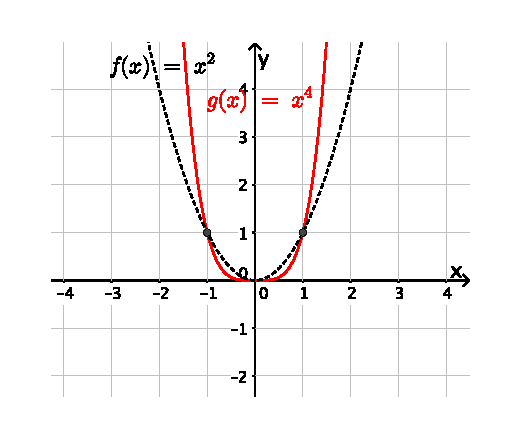
\includegraphics[width=73mm]{PotenzFktx2x4.pdf} &
  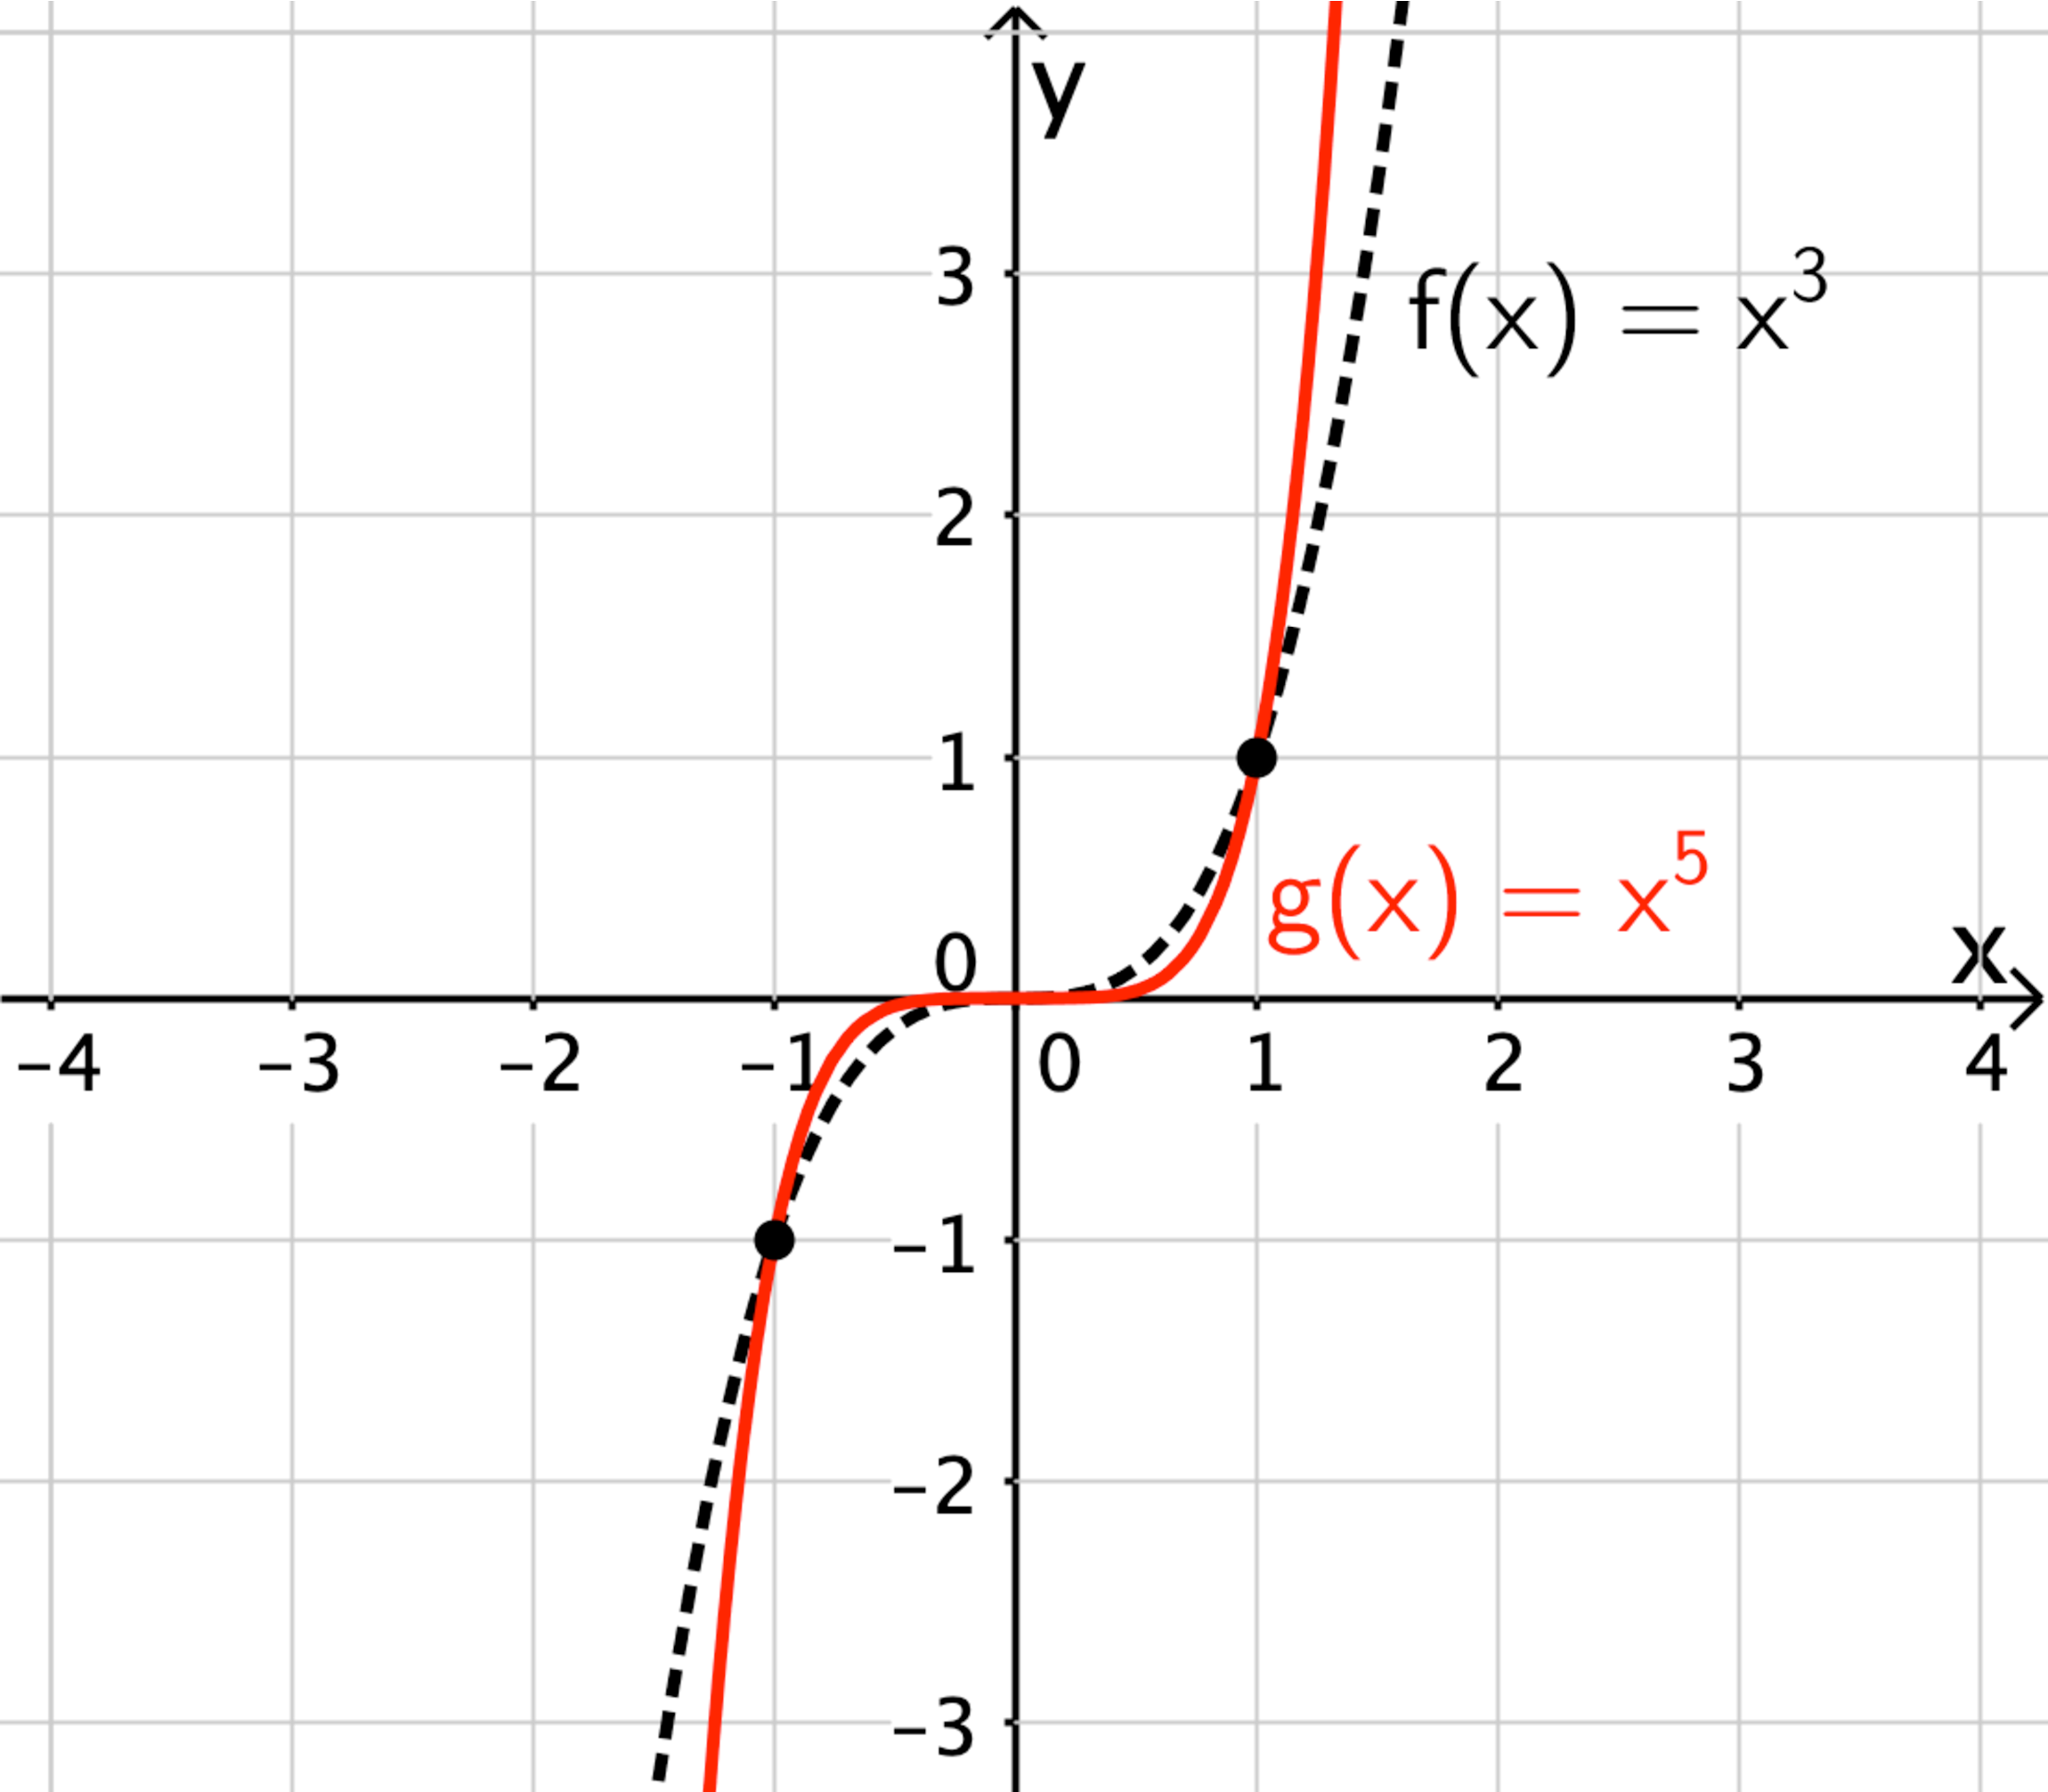
\includegraphics[width=73mm]{PotenzFktx3x5.pdf}\\

$k<0$: Hyperbel  ($k$ gerade) & $k<0$: Hyperbel ($k$ ungerade)\\
  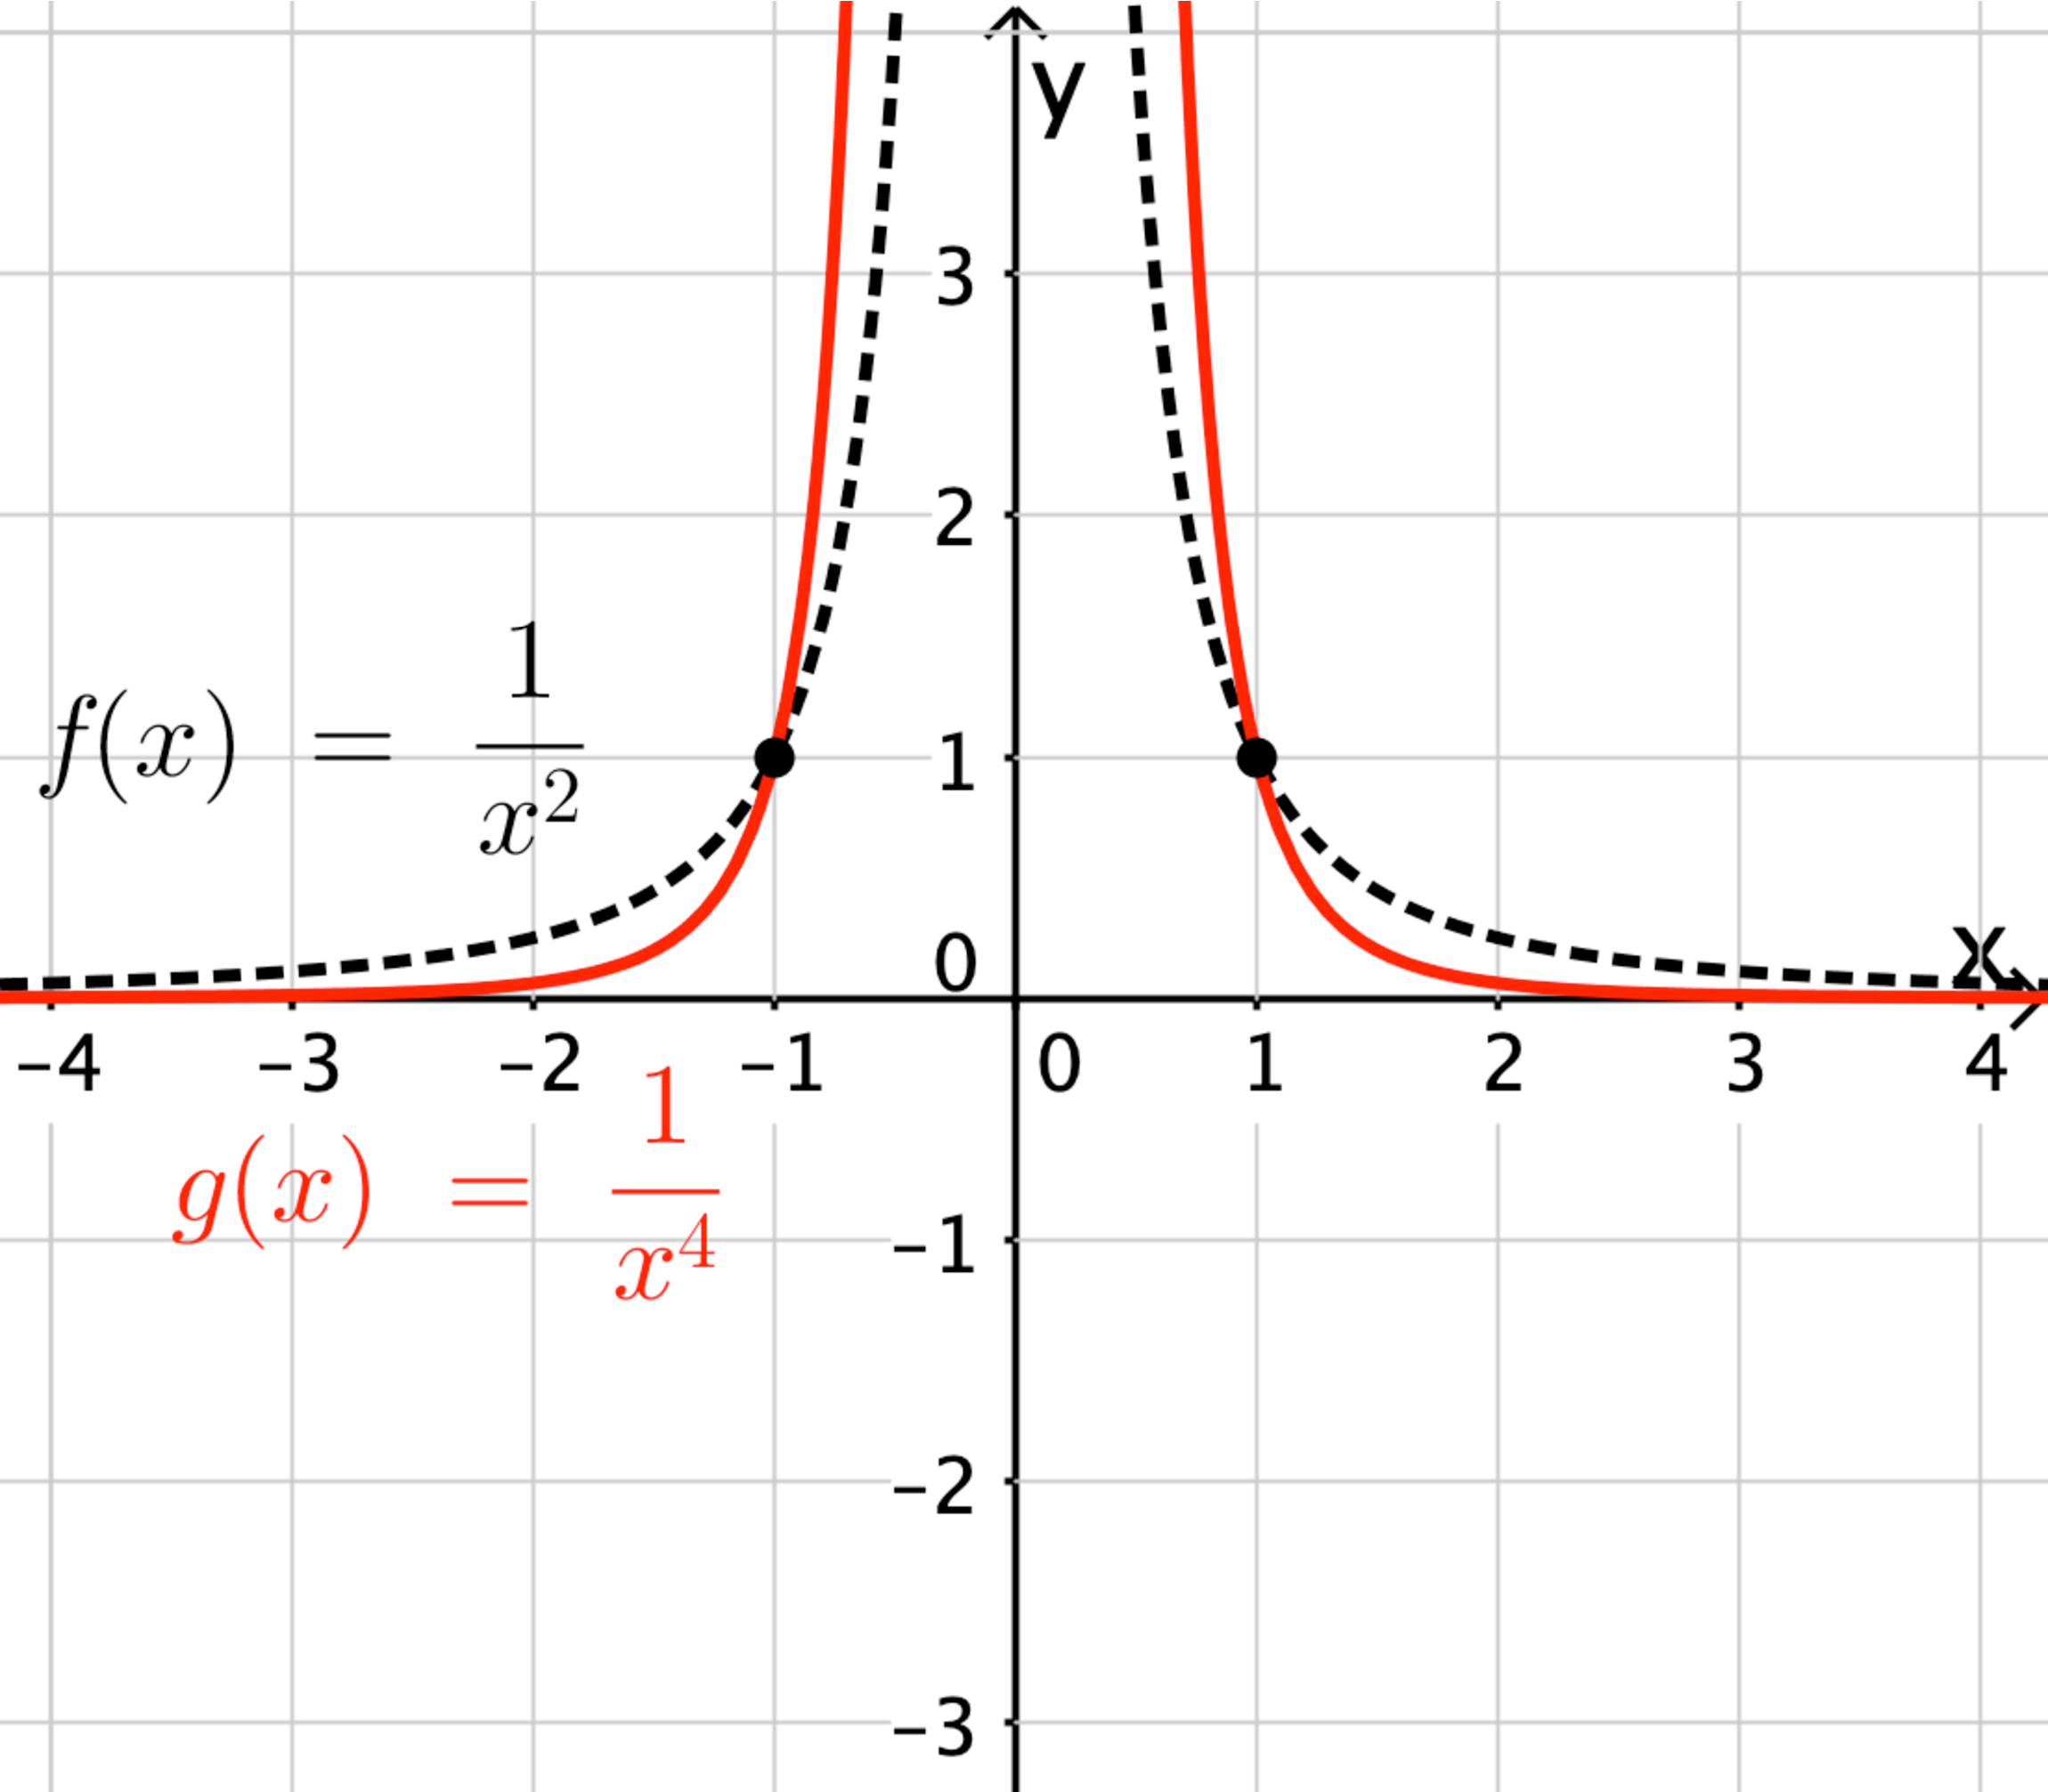
\includegraphics[width=73mm]{PotenzFkt1overx2x4.pdf}&
  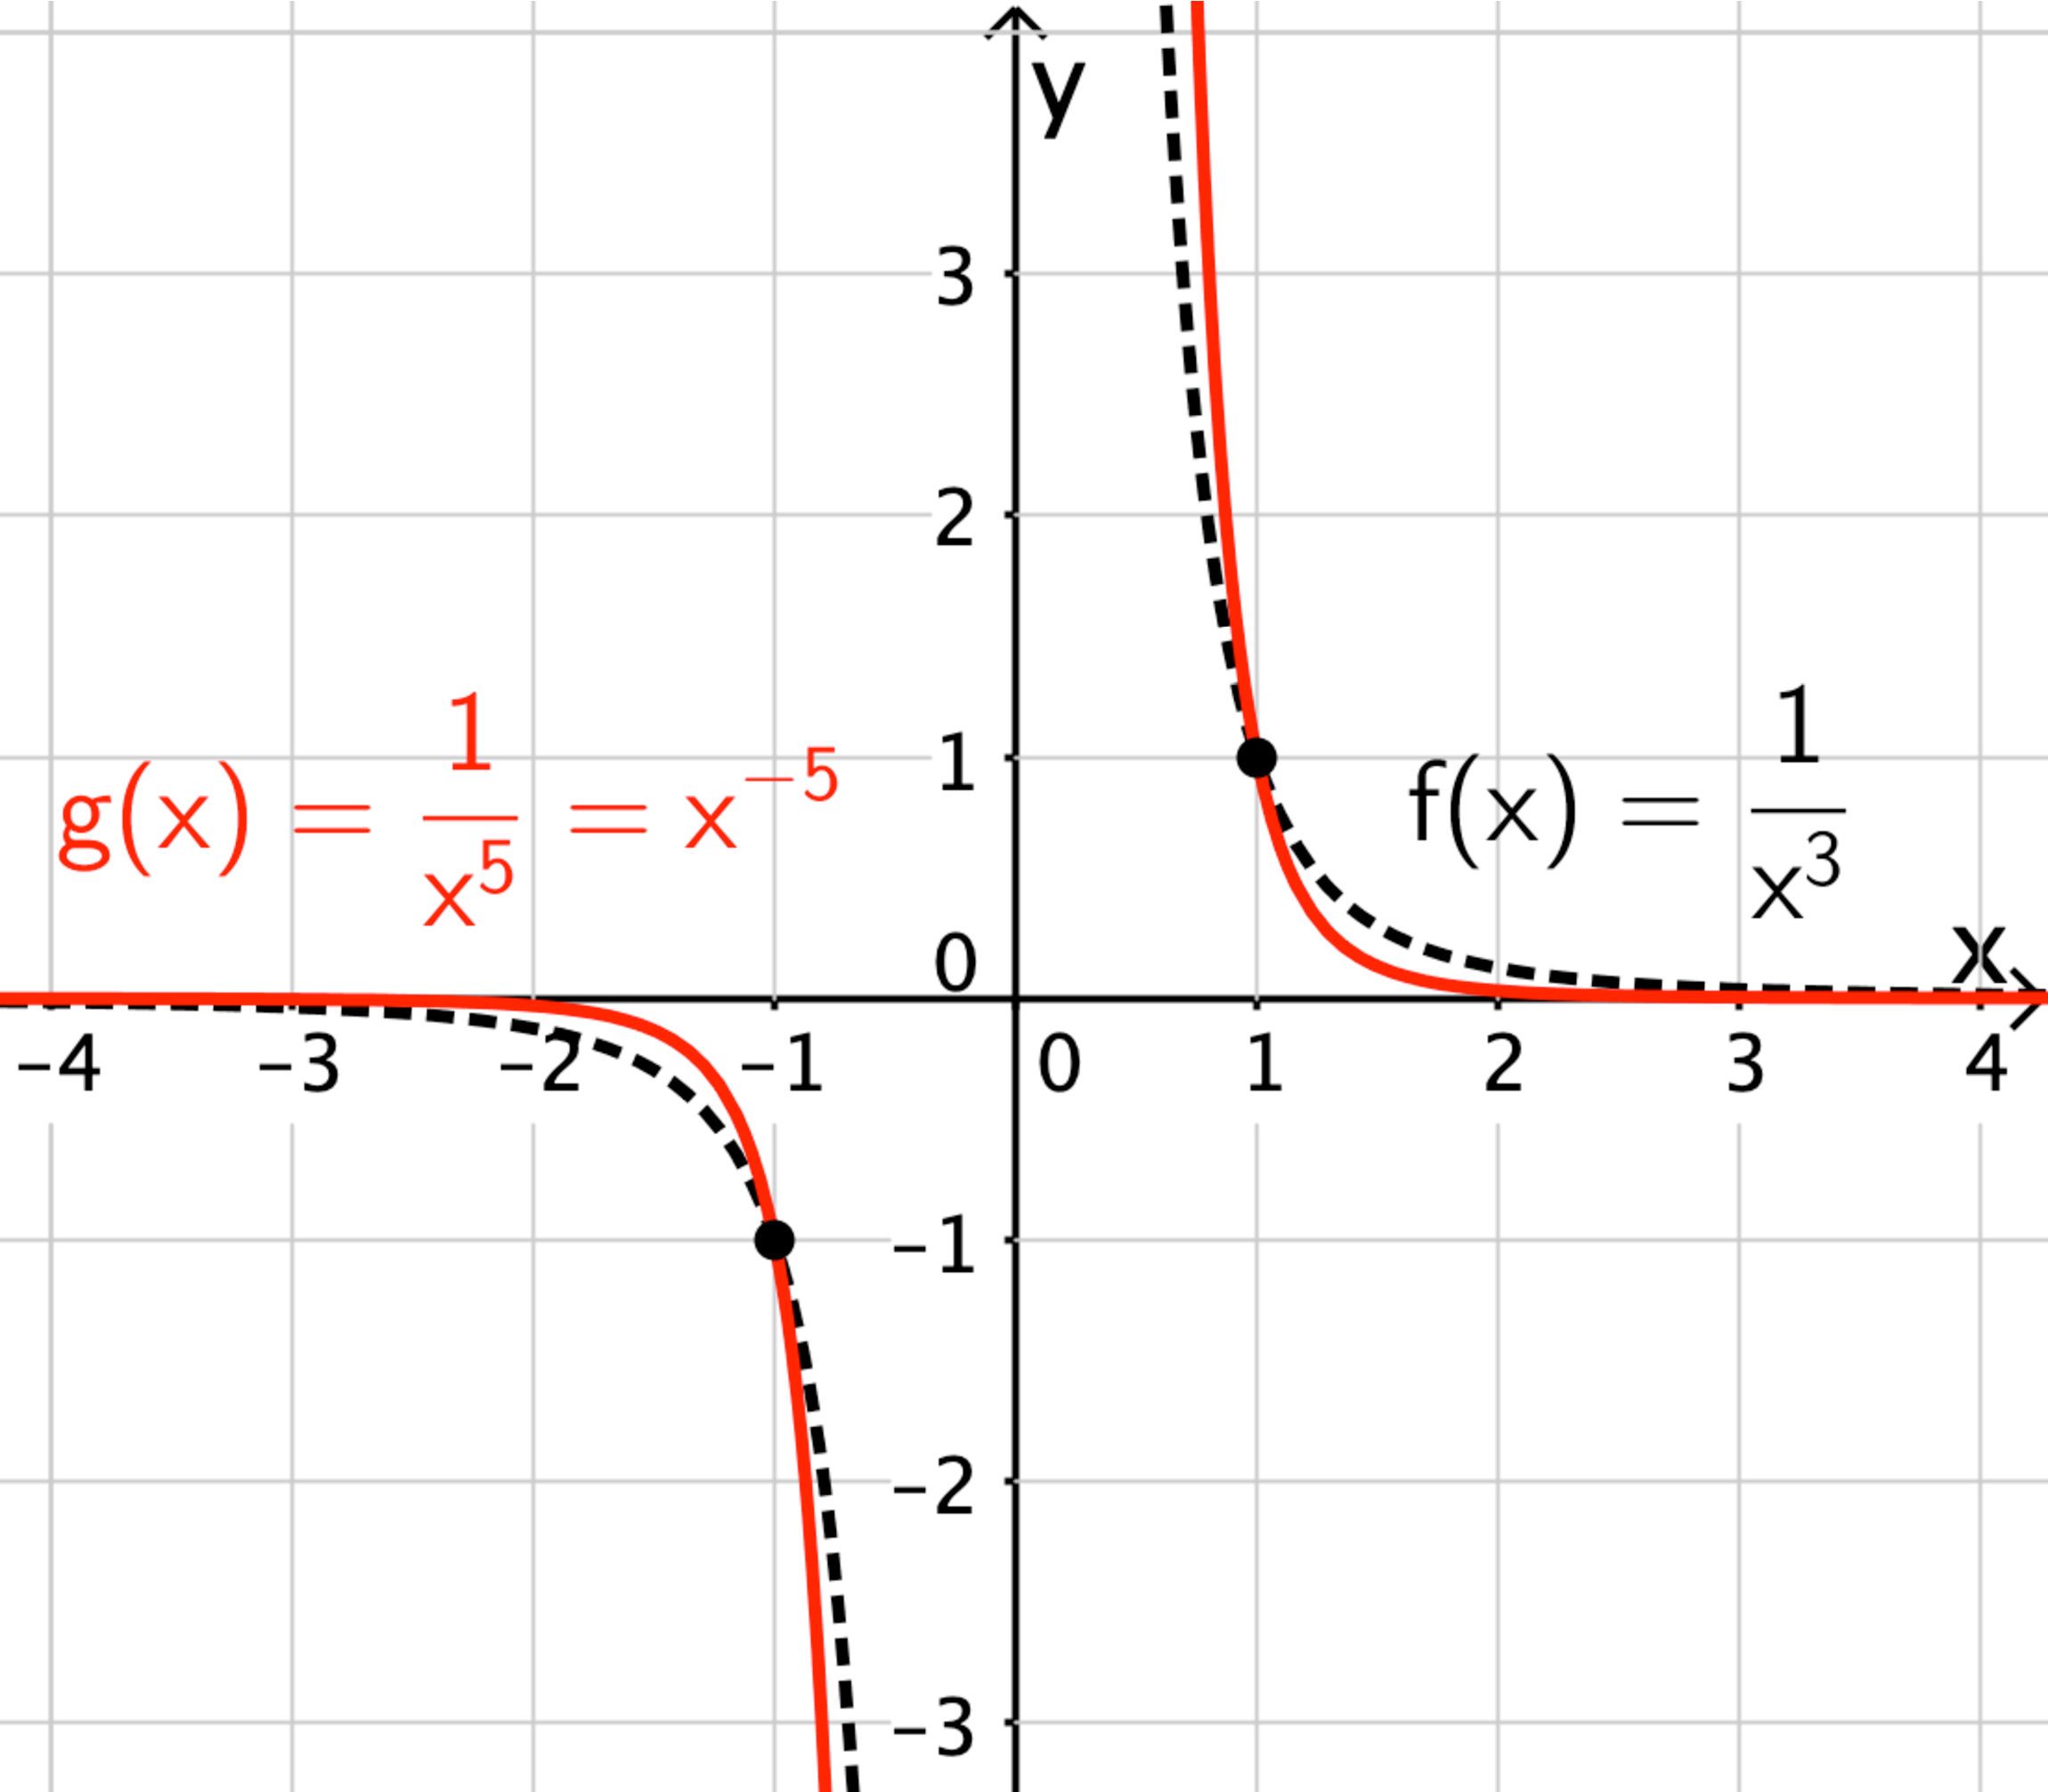
\includegraphics[width=73mm]{PotenzFkt1overx3x5.pdf}
  \end{tabular}


\begin{multicols}2

\begin{tcolorbox}[colback=white]
  \textbf{Grundform der Potenzfunktion}
$$y=ax^k$$
$k \in \{...-2, -1, 2, 3, 4, ...\}$
\end{tcolorbox}

$k$ gerade: Achsensymmetrisch ($y$-Achse)

$k$ ungerade: Punktsymmetrisch (Ursprung $O=(0|0)$)

%%Ist ${\color{green}a>0}$, so sind Graphen mit
%%geraden Exponenten nach oben geöffnet bzw. mit ungeraden Exponenten im
%%Quadranten I und III.

%%Ist ${\color{blue}a<0}$, so werden Graphen der obigen Funktionen an der $x$-Achse gespiegelt.

%% 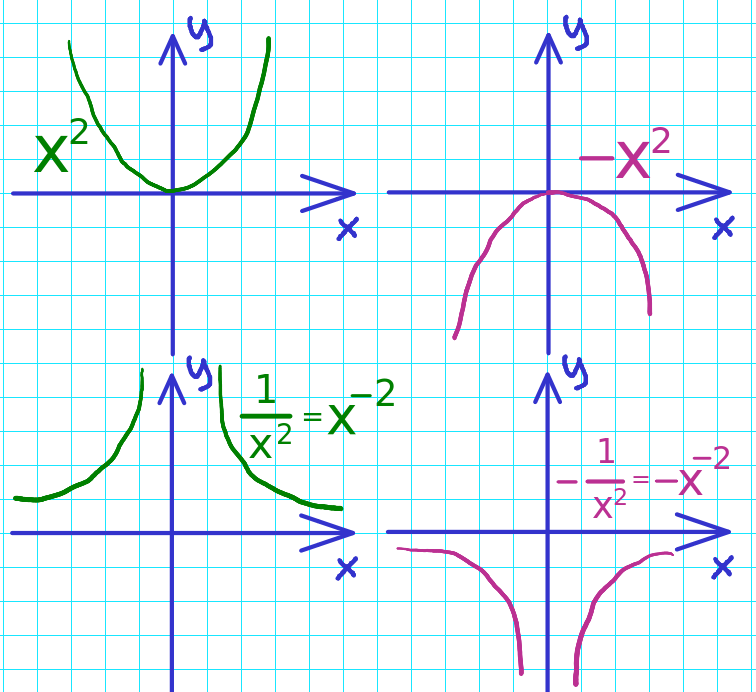
\includegraphics[width=4cm]{allg/funktionen/img/potenzfct/potenzFunktionenGerade.png}\hfill{}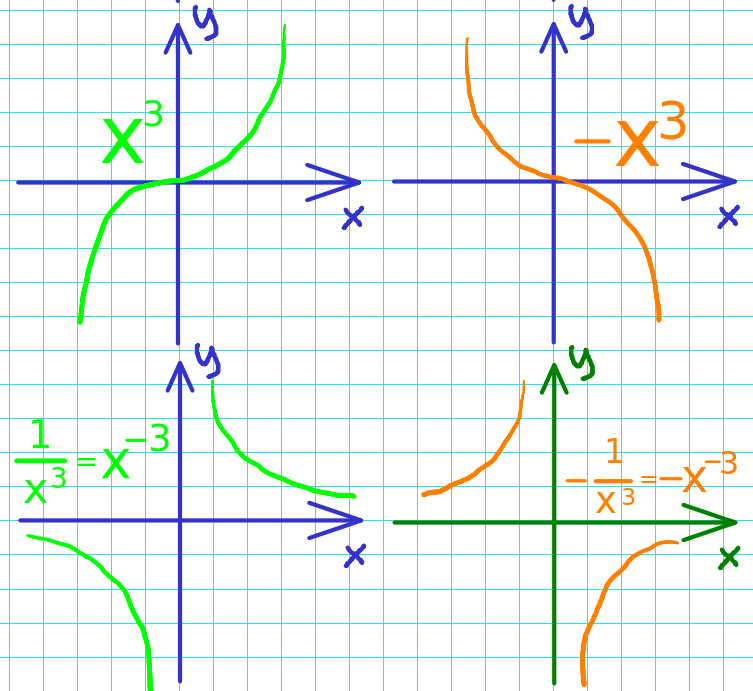
\includegraphics[width=4cm]{allg/funktionen/img/potenzfct/potenzFunktionenUngerade.png}
  \subsection*{Streckung / Spiegelung}
  Der Faktor $a$ in $y=a\cdot{}x^k$ streckt die Funktion in
  $y$-Richtung, bzw. spiegelt die Funktion an der $x$-Achse, wenn
  $a<0$ ist.
  \bbwCenterGraphic{73mm}{PotenzFktTransformation.pdf}



%%\hrulefill  
\forceCB
\keinHeaderUndKeinFooter{}

%%%%%%%%%%%%%%%%%%%%%%%%%%%%%%%%%%%%%%%%%%%%%%%%%%%%%%%%
%%               Wachstumsmodelle                     %%
%%%%%%%%%%%%%%%%%%%%%%%%%%%%%%%%%%%%%%%%%%%%%%%%%%%%%%%%
\section*{Wachstumsmodelle}

\textbf{Lineares Wachstum}
$$f(t) = \HECH{a}\RLP{m}\cdot t + \HECH{b}\RLP{q}$$
Bei linearem Wachstum wird pro Zeiteinheit der selbe Wert $\HECH{a}\RLP{m}$ \textbf{addiert}.

\textbf{Exponentielles Wachstum}

\HECH{$$f(t) = b\cdot{}a^t$$}
\RLP{$$f(t) = a\cdot{}q^t$$}
Bei exponentiellem Wachstum wird pro Zeiteinheit mit dem selben Wert $\HECH{a}\RLP{q}$ \textbf{multipliziert}.

  \begin{tabular}{rl}
   $\HECH{b}\RLP{a}$  & Startwert bei $t=0$; $\HECH{b}\RLP{a}=f(0)$\\
        & \phantom{$b$} = $y$-Achsenabschnitt\\
   $\HECH{a}\RLP{q}$  & beschreibt das Wachstum
  \end{tabular}

$$A_0 = A(0) = f(0); A_t = A(t) = f(t)$$

\HECH{\bbwCenterGraphic{8cm}{ExpFktVergleichMitLinearemWachstumHECH.pdf}}
\RLP{\bbwCenterGraphic{8cm}{ExpFktVergleichMitLinearemWachstumRLP.pdf}}

\subsection*{Exponentialfunktionen}
%%\bbwCenterGraphic{8.5cm}{allg/funktionen/img/exp/exponentielles_wachstum.png}
\begin{tcolorbox}[colback=white]$$y=f(t) = \HECH{b}\RLP{a}\cdot{}{\HECH{a}\RLP{q}}^t$$\end{tcolorbox}

Wachstum:
\HECH{$a>1$, Zerfall: $0<a<1$}
\RLP{$q>1$, Zerfall: $0<q<1$}


\begin{tcolorbox}[colback=white]
Wachstum bezogen auf eine Zeitspanne  
  $$f(t) = {\color{blue}\HECH{b}\RLP{a}}\cdot{}{\color{red}\HECH{a}\RLP{q}}^{\frac{t}{\color{FarnFarbe}\tau}}$$
  \begin{tabular}{ccp{60mm}}
$\color{FarnFarbe}\tau$ &=& Beobachtungsintervall zu $\color{red}\HECH{a}\RLP{q}$\\
    $\color{red}\HECH{a}\RLP{q}$ &=& Wachstums(bzw. Zerfalls)rate im Zeit\-raum $\color{FarnFarbe}\tau$
    \end{tabular}

Beispiel: Die Algen mit Startwert von ${\color{blue}3} \textrm{ m}^2$ ver{\color{red}vier}fachen
sich alle {\color{FarnFarbe}fünf} Tage:\\
${\color{blue}\HECH{b}\RLP{a}}={\color{blue}3}$, ${\color{red}\HECH{a}\RLP{q}}={\color{red}4}$, ${\color{FarnFarbe}\tau}={\color{FarnFarbe}5}$
$$f(t)= {\color{blue}3}\cdot{}{\color{red}4}^\frac{t}{\color{FarnFarbe}5}$$
\end{tcolorbox}
\RLP{\bbwCenterGraphic{8cm}{ExponentialfctAQ.png}}
\HECH{\bbwCenterGraphic{8cm}{ExponentialfctAB.png}}

\subsection*{Basis $e$, Zeitvariable $x$}
$e$ = Eulersche Konstante $\approx 2.71828$
\HECH{$$y=b\cdot{}a^x$$ entspricht
$$y=b\cdot{}e^{mx}$$}

\RLP{$$y=a\cdot{}q^x$$ entspricht
$$y=a\cdot{}e^{bx}$$}

%\HECH{$\textrm{mit } m = \ln(a)\,\,\textrm{ oder } a = e^m$}
%\RLP{$\textrm{mit } b = \ln(q)\,\,\textrm{ oder } q = e^b$}
\HECH{$\textrm{mit } a = e^m \,\,\textrm{ oder }  m = \ln(a)$}%
\RLP{$\textrm{mit }  q = e^b \,\,\textrm{ oder }  b = \ln(q)$}%

\vspace{2mm}

\hrulefill

Und mit Zeitintervall $\tau$:

\HECH{$$y=b\cdot{}a^\frac{x}\tau$$ entspricht
$$y=b\cdot{}e^{mx}$$}
\RLP{$$y=a\cdot{}q^\frac{x}\tau$$ entspricht
$$y=a\cdot{}e^{bx}$$}

\HECH{$\textrm{mit } a = e^{m\tau}  \,\,\textrm{ oder }    m=\ln\left(a^\frac1\tau\right) = \frac1\tau \cdot{}\ln(a)$}
\RLP{$\textrm{mit }  q = e^{b\tau}  \,\,\textrm{ oder }    b=\ln\left(q^\frac1\tau\right) = \frac1\tau \cdot{}\ln(q)$}

\hrulefill
\subsection*{Halbwertszeit}
\HECH{$\frac12 \cdot{} b = f(t) = b\cdot{}a^{\frac{t}{\tau}}\phantom{xxx}\Longrightarrow\phantom{xxx}t= \tau\cdot{}\log_a\left(\frac12\right)$}
\RLP{$\frac12 \cdot{} a = f(t) = a\cdot{}q^{\frac{t}{\tau}}\phantom{xxx}\Longrightarrow\phantom{xxx}t= \tau\cdot{}\log_q\left(\frac12\right)$}

\keinHeaderUndKeinFooter{}

\subsection*{Verdopplungszeit}
\HECH{$2\cdot{}b = f(t) = b\cdot{}a^{\frac{t}{\tau}}\phantom{xxx}\Longrightarrow\phantom{xxx}t = \tau\cdot{}\log_a(2)$}
\RLP{$2\cdot{}a = f(t) = a\cdot{}q^{\frac{t}{\tau}}\phantom{xxx}\Longrightarrow\phantom{xxx}t = \tau\cdot{}\log_q(2)$}

%%\mmPap{5.6}%
\forceCB%
\keinHeaderUndKeinFooter{}



\subsection*{Sättigungsfunktionen}
\keinHeaderUndKeinFooter{}


\bbwCenterGraphic{7.5cm}{img/ExpFunktionBeschraenktesWachstum.pdf}

\subsubsection*{Beschränktes Wachstum (Zerfall)}
\keinHeaderUndKeinFooter{}


\textbf{Zerfallsrate} immer: $0<\HECH{a}\RLP{q}<1$

\textbf{Sättigungsgrenze}: $c$


\textbf{Zerfall}:
\HECH{$$f(t) = c+b\cdot{}a^\frac{t}\tau$$
$$f(0) = c+b$$}
\RLP{$$f(t) = c+a\cdot{}q^\frac{t}\tau$$
$$f(0) = c+a$$}


\textbf{Wachstum}:

\HECH{$$f(t) = c-b\cdot{}a^\frac{t}\tau$$
$$f(0) = c-b$$}
\RLP{$$f(t) = c-a\cdot{}q^\frac{t}\tau$$
$$f(0) = c-a$$}

%%\textbf{Sättigungsdefizit}
%%$b$ = Differenz zu $c$ bei $t=0$.\\
%%$b\cdot{}a^\frac{t}\tau = m(t)$ = Sättigungsdefizit zur Zeit $t$

\end{multicols}

%%\mmPapier{14}

\newpage
\keinHeaderUndKeinFooter{}

%%%%%%%%%%%%%%%%%%%%%%%%%%%%%%%%%%%%%%%%%%%%%%%%%%%%%%%%
%%               Datenanalyse                         %%
%%%%%%%%%%%%%%%%%%%%%%%%%%%%%%%%%%%%%%%%%%%%%%%%%%%%%%%%
\section*{Datenanalyse}
\HECH{\bbwCenterGraphic{17cm}{img/Skalentyp.pdf}
\vspace{5mm}}%% END  HECH
%%\bbwCenterGraphic{15cm}{img/DatenanalyseSkalentypen.eps}
\HECH{\hrulefill}

\begin{multicols}{2}

\subsection*{Lagemasse}


\subsubsection*{Modus\TRAINER{, Modalwert?}}
Der am häufigsten auftretende Wert wird als Modus bezeichnet.

Manchmal ist dies nicht eindeutig, dann sprechen wir von einer
\textbf{multimodalen} Verteilung; bei zwei Modi von \textbf{bimodal}.


\subsubsection*{Mittelwert}
(= Durchschnitt = arithmetisches Mittel)

$$\overline{x} = \frac{x_1 + x_2 + x_3 + ... +
x_n}{n}=  \frac{\sum\limits_{k=1}^nx_n}n$$

\subsubsection*{Median}


Der \textbf{Median} (Zentralwert) ist der Wert in der Mitte der geordneten Datenreihe. Ist
die Anzahl Werte gerade, so wird der Mittelwert der beiden
«mittleren» Werte genommen.

Symbol: $\mediantilde{x} = x_{\textrm{MED}}$


\subsubsection*{Quartil}

Die Quartilsgrenzen $Q_1$ bzw. $Q_3$ sind die Mediane der linken,
bzw. rechten Datenhälfte (nachdem der eine Zentralwert entfernt
wurde).

\subsubsection*{Maximum, Minimum}

Maximum bzw. Minimum sind höchste bzw. kleinste Datenwerte: Die Ausreisser
zählen mit!

\RLP{\forceCB}%%
\keinHeaderUndKeinFooter{}

%%%%%%%%%%%%%%%%%%%%%%%%%%%%%%%%%%%%%%%%%%%%%%%%%%%%%%%%%5

\subsection*{Streumasse}
\subsubsection*{Spannweite}
Die Spannweite $R$ (Range) ist das Maximum minus
das Minimum.
\subsubsection*{Standardabweichung}
Mit $\sigma$ bzw. $s$ wird die Standardabweichung bezeichnet. Es ist
ein Mass für die Streuung um den Mittelwert.


\subsubsection*{Interquartilsabstand}
Der Abstand zwischen $Q_1$ und $Q_3$ wird als
Quartilsdifferenz \textbf{QD} oder
englisch \textit{Inter Quartile Range} = \textbf{IQR} bezeichnet.


%$\sigma$ = Standardabweichung der Grundgesamtheit

%$s$ = Standardabweichung einer gemessenen Stichprobe
\keinHeaderUndKeinFooter{}


\subsubsection*{Robustheit}
Verändert sich der Wert eines statistischen Masses nicht, wenn sich ein Ausreisser
weiter ins Extreme bewegt, so sprechen wir von einem \textbf{robusten} Mass.

\begin{tabular}{|c|l|l|}\hline
   & Lage- & Streumass\\\hline
 \multirow{4}{*}{\rotatebox{90}{robust}}  & Median $\mediantilde{x}$ & IQR \\
    & Modus $x_{mod}$ & \\
    & Quartile ($Q_1$,$Q_3$) & \\
    & (Ausreisserschwellen) & \\\hline
 \multirow{3}{*}{\rotatebox{90}{«fragil»}}  & Mittelwert
 $\overline{x}$ & Spannweite\\
    & Minimum & Standardabw.: $\sigma$\\

 & Maximum & \\\hline
 \end{tabular}



%
\keinHeaderUndKeinFooter{}

\RLP{\forceCB}%
\keinHeaderUndKeinFooter{}

\subsection*{Diagramme}
\keinHeaderUndKeinFooter{}

\subsubsection*{Säulen (und Balken) / Kreis (Kuchen)}
\keinHeaderUndKeinFooter{}

%%\begin{tabular}{cc}
%% 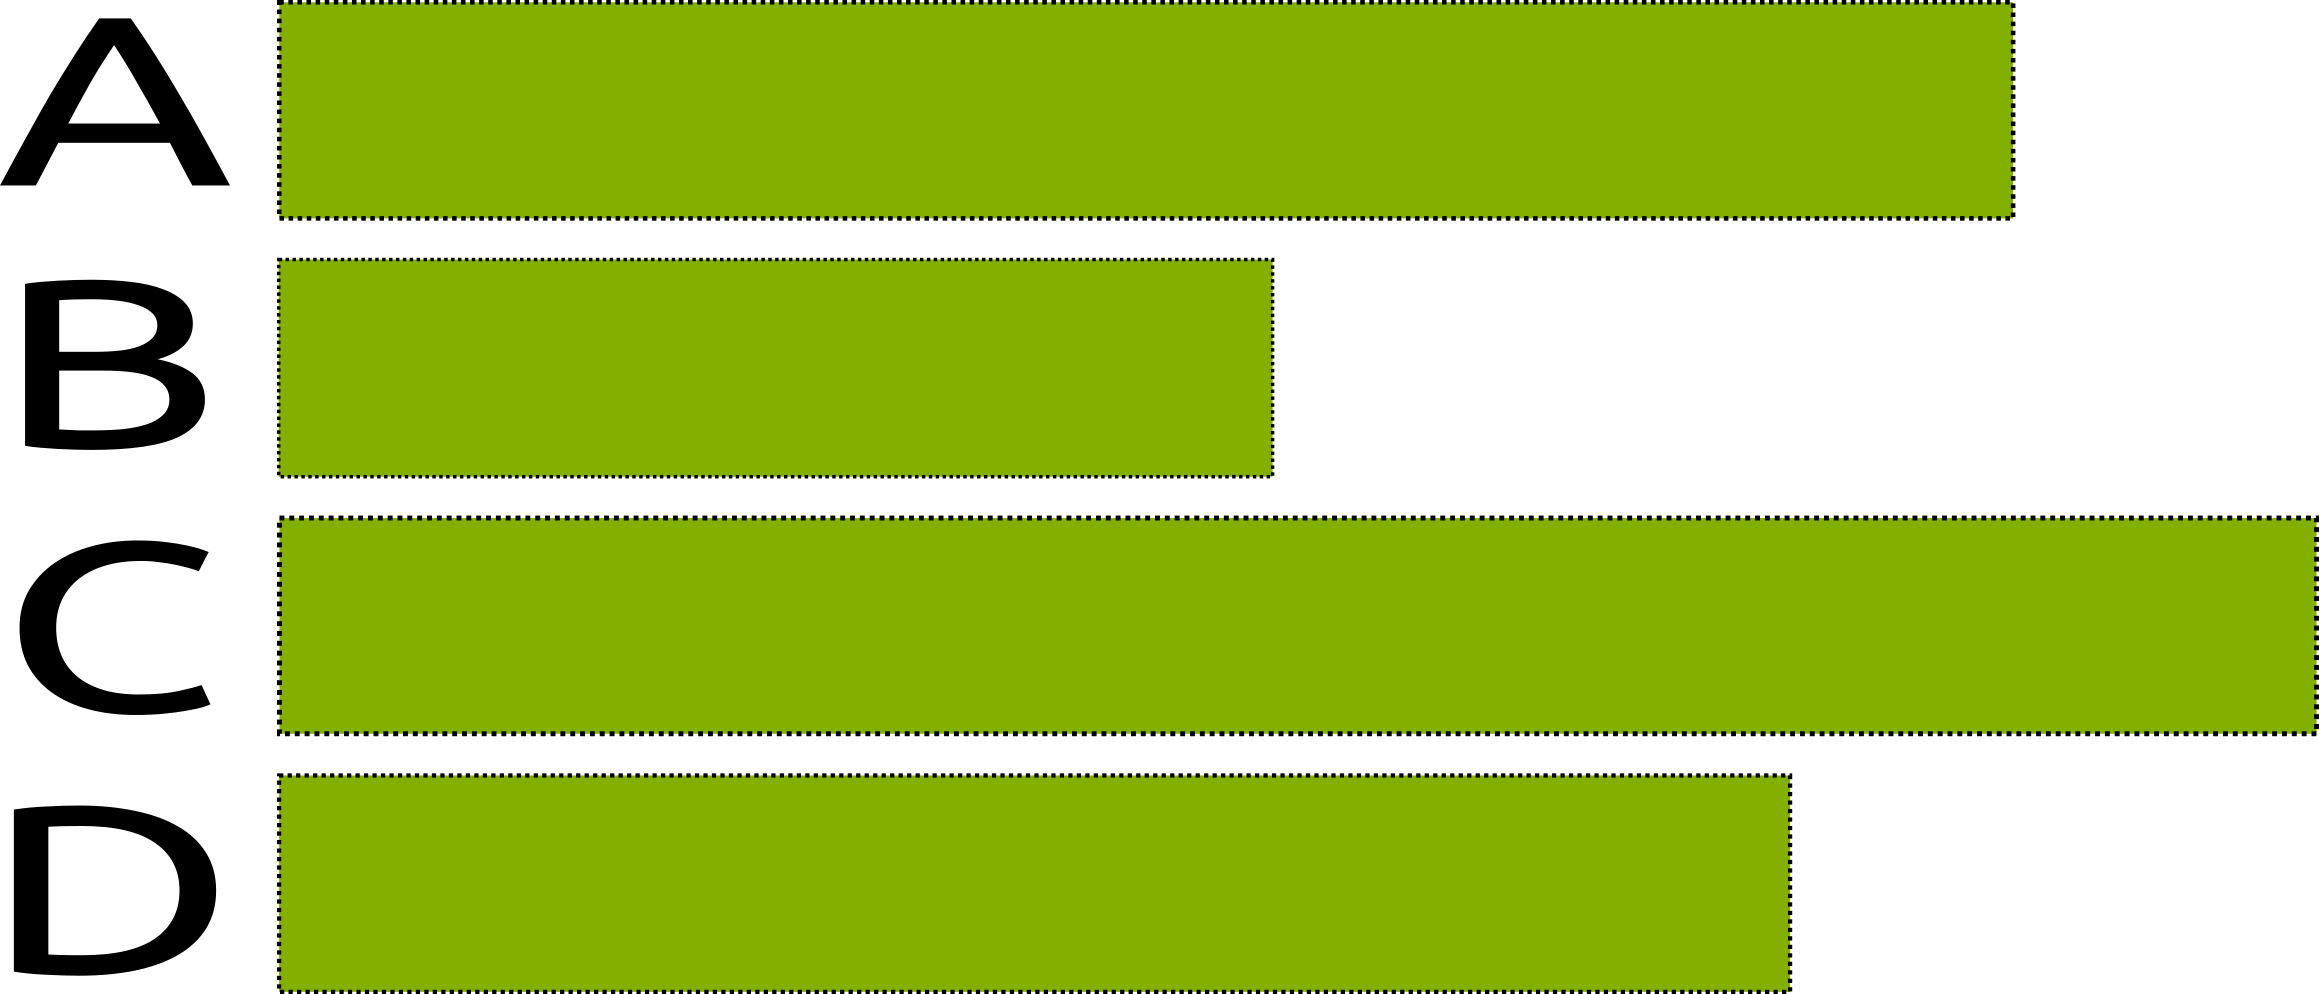
\includegraphics[width=4cm]{img/balkendiagramm.png} &  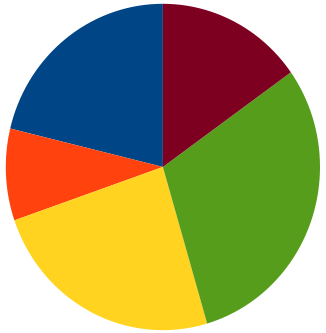
\includegraphics[width=3cm]{img/kuchendiagramm.png}\\
%%\end{tabular}

\begin{itemize}
\item Säulen- und Kreisdiagramme werden für ordinale und nominale
  Skalen verwendet (und bei quantitativ diskreten Datentypen, wenn es
  nur wenige Ausprägungen sind).
\item Achse: Unverzerrte Skalierung und Beschriftung
\item Legende und Titel
\end{itemize}

\keinHeaderUndKeinFooter{}

\begin{tcolorbox}[colback=white]
  \textbf{Absolute und relative Häufigkeit}\\
\begin{tabular}{lcl}

$n$   &$=$& Anzahl Werte\\
$h_i$ &$=$& Absolute Häufigkeit\\
      & & des Merkmals $i$\\
$f_i = \frac{h_i}n$ &$=$& relative Häufigkeit\\
$p_i = f_i\cdot{}100\%$ &$=$& prozentuale Häufigkeit%%\\
%%$\varphi_i = f_i\cdot{}360\degre$ &$=$& Zentriwinkel im\\
%%      & &Kuchendiagramm
  \end{tabular}
\end{tcolorbox}

\keinHeaderUndKeinFooter{}

\RLP{\forceCB}

\keinHeaderUndKeinFooter{}

\subsubsection*{Histogramm}
\keinHeaderUndKeinFooter{}
\bbwCenterGraphic{8cm}{img/Histogramm.pdf}

\begin{itemize}
\item Alle Balken sind gleich breit und berühren sich.
\item Die Höhe der Balken wird durch die (absolute / relative) Häufigkeit der entsprechenden
  Werte festgelegt.
\item Die Flächeninhalte der Rechtecke sind proportional
  zu den Häufigkeiten.
\item Werte auf Balkengrenzen werden immer rechts mitgezählt.
\item Das obige Histogramm ist \textbf{linksschief} und rechtssteil.
\end{itemize}


%Vorgehen
%\begin{enumerate}
%\item Daten in TR eingeben \tiprobutton{data}...
%\item ... und mit \tiprobutton{2nd} \tiprobutton{data_stat-reg-distr} auslesen.
%\item {\color{orange} Median ($\mediantilde{x} = x_{\textrm{MED}}$)},
%und Quartile ({\color{blue}$Q_1$}, {\color{FarnFarbe}$Q_3$})einzeichnen
%\item IQR := {\color{FarnFarbe}Q3}-{\color{blue}Q1} rechnen
%\item IQR mit 1.5 multiplizieren
%\item {\color{red} untere Ausreisserschwelle\\ uAs} $ = Q_1 -
%1.5\cdot{}\textrm{IQR}$\\ und {\color{red} obere Ausreisserschwelle\\ oAs} $=Q_3 + 1.5\cdot{}\textrm{IQR}$\\ (ausradierbar) fein markieren (gehören nicht zum Boxplot)
%\item Alle Ausreisser mit Ring $\circ$ oder Stern $\star$ einzeichnen.
%\item Whisker (entfernteste Werte innerhalb der Ausreisserschwellen)
%einzeichnen.
%\item Boxdekoration horizontale Linien einzeichnen.
%\end{enumerate}
%\bbwCenterGraphic{8cm}{img/Boxplot.pdf}

\end{multicols}


\keinHeaderUndKeinFooter{}
\newpage
\keinHeaderUndKeinFooter{}
\subsubsection*{Boxplot}
%%\TRAINER{«Schritte zum Boxplot als Fliesstext
%%  daneben. Ausreisserschwellen {\color{blue}blau} im
%%  Diagramm. Dann im Text auch. Ausreisserschwellen ist ein Begriff von
%%  Frommenwiler, nicht von Marthaler.}%% END TRAINER
Schritte zum Boxplot:\\
Fühler (Whisker) werden auf max. $1.5\cdot\textrm{IQR}$ begrenzt ({\color{blue} Ausreisserschwellen blau})\HECH{,
danach nach \textit{\color{FarnFarbe}innen} gehen}: Fühler sind die von der Box
entferntesten Nicht-Ausreisser ({\color{FarnFarbe}grün}). Ausreisser
({\color{red} rot}) werden markiert.
\RLP{\bbwCenterGraphic{18cm}{boxplotRLP.png}}
\HECH{\bbwCenterGraphic{18cm}{boxplotHECH.png}}
%%\TRAINER{Entferne «Sportler*innen»}

\hrulefill

\begin{multicols}{2}
%%%%%%%%%%%%%%%%%%%%%%%%%%%%%%%%%%%%%%%%%%%%%%%%%%%%%%%%
%%    Kombinatorik / Wahrscheinlichkeit (Stochastik)  %%
%%%%%%%%%%%%%%%%%%%%%%%%%%%%%%%%%%%%%%%%%%%%%%%%%%%%%%%%
\section*{Stochastik}
\keinHeaderUndKeinFooter{}

\subsection*{Kombinatorik}

\subsubsection*{Produktregel}

\begin{tabular}{p{5cm}c}
Bsp.: Andrea hat drei verschiedene Hosen und vier verschiedene Pullover.
Es gibt somit $3\cdot{}4$ mögliche Kombinationen.&\raisebox{-3.5cm}{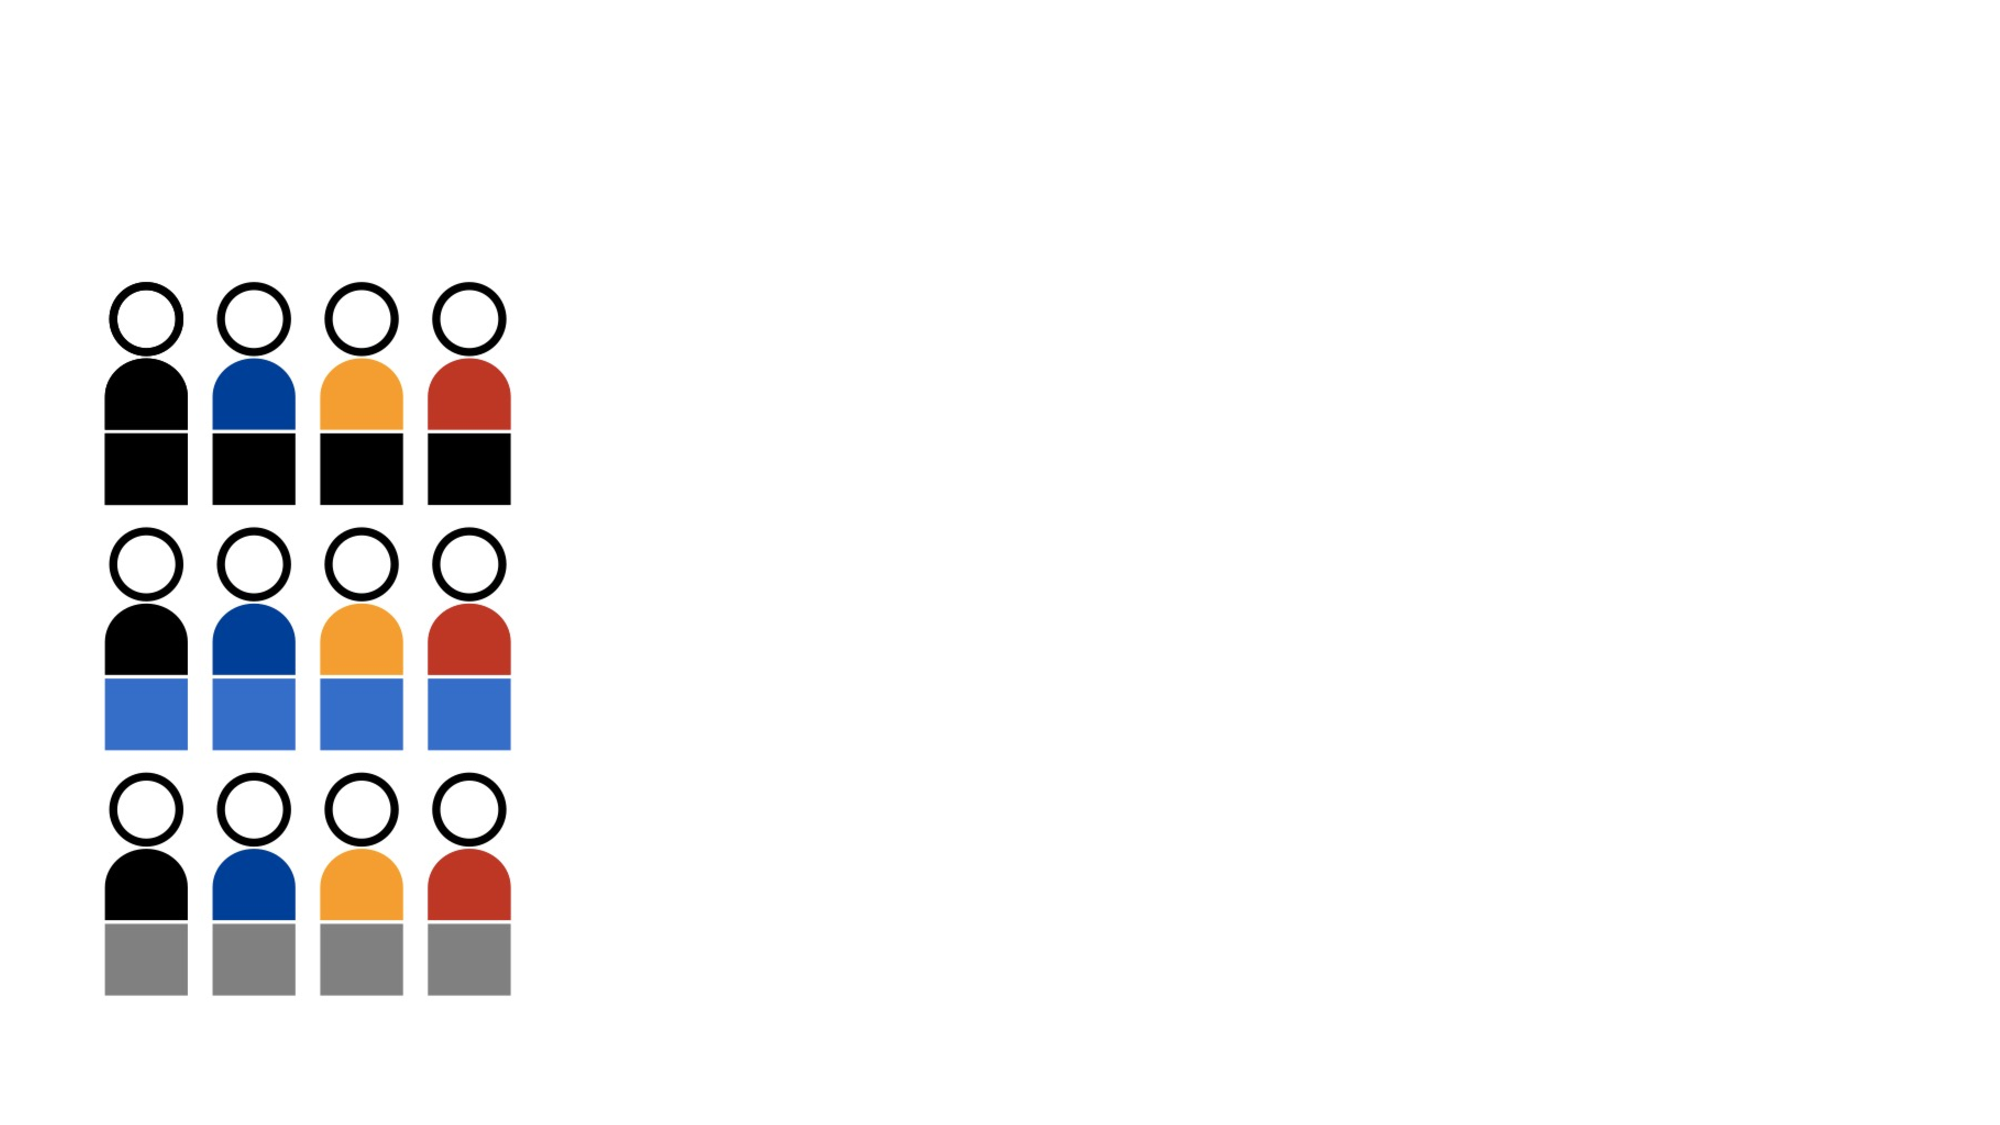
\includegraphics[width=3cm]{img/KombinatorikMultiplikation.pdf}}\end{tabular}


Hat eine zweistufige Situation zunächst $k_1$ Möglichkeiten, gefolgt
von $k_2$ Möglichkeiten, so hat man insgesamt $k_1\cdot{}k_2$
Möglichkeiten. Dies ist auf beliebig viele Stufen verallgemeinerbar.



%%\bbwCenterGraphic{3cm}{img/KombinatorikMultiplikation.pdf}
%%\TRAINER{Ersetze «Ein:e Schüler:in» durch «Andrea»}
\forceCB
\subsubsection*{Permutationen (Sitzordnungen)}

Bei $n$ Elementen gibt es $n!$ Permutationen (=Vertauschungen):
                                                                                                                
\begin{tcolorbox}[colback=white]
  \textbf{Fakultät}\\
  $$n! = n\cdot{}(n-1)\cdot{}(n-2)\cdot{}(n-3)\cdot{} ... \cdot{}2\cdot{}1$$
  $$1! = 1\phantom{xxx}0! = 1$$
\end{tcolorbox}



\def\missifarbig{M{\color{FarnFarbe}i}{\color{red}ss}{\color{FarnFarbe}i}{\color{red}ss}{\color{FarnFarbe}i}{\color{cyan}pp}{\color{FarnFarbe}i}}

\vspace{3mm}
\textbf{Permutation mit Wiederholung}

oder «\missifarbig»-Formel: Sind bei einer Permutation (Vertauschung) einige Elemente gleich, so reduziert
sich die Anzahl der Möglichkeiten. Wie viele verschiedene Wörter sind mit den Buchstaben des Wortes «\missifarbig» bildbar?
$$N = \frac{11!}{{\color{FarnFarbe}4}!\cdot{}{\color{red}4}!\cdot{}{\color{cyan}2}!}$$




\end{multicols}
\newpage
\keinHeaderUndKeinFooter{}


\subsection*{Überblick Auswahlprobleme / Anzahl Möglichkeiten $N$ }

$$\textrm{Binomialkoeffizient:} {{\color{blue}n}\choose
{\color{red}k}}
=\frac{{\color{blue}n}!}{({\color{blue}n}-{\color{red}k})!\cdot
{\color{blue}n}!}\phantom{etwas Platz lassen} {n\choose 0}= {n\choose
n}= 1$$

\RLP{\bbwCenterGraphic{17cm}{img/KombinatorikRLP.pdf}}
\HECH{\bbwCenterGraphic{17cm}{img/KombinatorikHECH.pdf}}

\hrulefill



\begin{multicols}{2}


\subsection*{Wahrscheinlichkeit}
\subsubsection*{Grundbegriffe}

\textbf{Ergebnismenge} $\Omega$: Menge der möglichen Ergebnisse
(Ausgänge) eines Zufallsversuchs.\\
Beispiel: Die sechs Würfelergebnise
eines Spielwürfels: $\Omega = \left\{\epsdice{1}, \epsdice{2}, \epsdice{3}, \epsdice{4}, \epsdice{5}, \epsdice{6}\right\}$

\textbf{Ereignis} $A$: Eine Teilmenge von $\Omega$. Beispiel: Eine
ungerade Zahl zu werfen: $A  = \left\{\epsdice{1}, \epsdice{3}, \epsdice{5}\right\}$

\textbf{Gegenereignis} $\overline{A} = \Omega \backslash A$ =
\textit{Gegenmenge}

$\overline{A}$ sprich «nicht» $A$.

Es gilt $A \cup \overline{A} = \Omega$

\textbf{Elementarereignis}: Ereignis bestehend aus einem einzigen
Ergebnis aus $\Omega$. Beispiel: $E_1$ = Wirf eine \textbf{Eins}: $E_1
= \left\{\epsdice{1}\right\}$.

\forceCB


\subsection*{Laplace-Wahrscheinlichkeit}
Sind alle möglichen Ergebnisse eines Zufallsversuchs gleich
wahrscheinlich (fairer Würfel), so ist die Wahrscheinlichkeit $P(E)$ für das Ereignis
$E$ wie folgt zu berechnen:

$$P(E) = \frac{\textrm{Anzahl Ergebnisse in
}E}{\textrm{Anzahl Ergebnisse in }\Omega}$$

\forceCB
\subsubsection*{Baumdiagramme}
Bsp.: Zwei Mal eine \textit{unfaire} Münze werfen
\bbwCenterGraphic{75mm}{img/WahrscheinlichkeitBaumdiagramm.pdf}

Wahrscheinlichkeiten {\color{FarnFarbe}entlang} eines Pfades werden {\color{FarnFarbe}multipliziert}:
$$P(KK) = 0.6\cdot0.6=0.36$$

Wahrscheinlichkeiten {\color{red}verschiedener} Pfade werden
{\color{red}addiert}:

\begin{tabular}{rcl}
${\color{red}P}({\color{FarnFarbe}KK} \textrm{\color{red} oder } {\color{blue}ZZ})$ &=&
  $P({\color{FarnFarbe}KK}) {\color{red}+} P({\color{blue}ZZ})$\\
  &=&${\color{FarnFarbe}0.6\cdot0.6} {\color{red}+} {\color{blue}0.4\cdot0.4}$
\end{tabular}
 
\keinHeaderUndKeinFooter{}

\subsection*{Binomialverteilung (Bernoulli)}
\keinHeaderUndKeinFooter{}

Voraussetzung: Es gibt pro Verzweigung nur zwei Ausgänge mit jeweils
gleicher Trefferwahrscheinlichkeit.


\begin{tcolorbox}[colback=white]
$$P(X=k) = {n \choose k}\cdot{}p^k\cdot{}(1-p)^{n-k}$$
$k$ = \textbf{genaue} gewünschte Anzahl Treffer\\
$n$ = Anzahl Züge\\
$p$ = Wahrscheinlichkeit des Treffers\\
Taschenrechner:  \textbf{\texttt{binomialpdf}}
\end{tcolorbox}%%

Beispiel: Ein Ballspieler trifft mit 35\% Wahrscheinlichkeit
($p=0.35$). Wie gross ist die Wahrscheinlichkeit, dass er mit 20 Würfen
($n=20$) \textbf{genau} vier Mal ($k=4$) trifft?

Lösung: \texttt{binomialpdf} $\Longrightarrow 7.38\%$



\subsubsection*{Kumulierte Binomialverteilung}

\begin{tcolorbox}[colback=white]
$$P(X\le k) = \sum_{i=0}^{k}{n \choose i}\cdot{}p^i\cdot{}(1-p)^{n-i}$$
$k$ = \textbf{maximal} gewünschte Anzahl Treffer\\
$n$ = Anzahl Züge\\
$p$ = Wahrscheinlichkeit des Treffers\\
Taschenrechner: \textbf{\texttt{binomialcdf}}
\end{tcolorbox}


\subsection*{Hypergeometrische Verteilung\\ (Lottomodell)}
\begin{tcolorbox}[colback=white]
Gegeben $N+T$ Kugeln in einer Urne. Herausgezogen werden $n+t$:
\begin{itemize}
\item $T$ Anzahl aller Treffer
\item $N$ Anzahl aller Nieten
\item $t$ gewünschte Treffer
\item $n$ «gewünschte» Nieten
\end{itemize}
Wahrscheinlichkeit \textbf{genau} $t$ Treffer zu ziehen:

$$P_{N,T,n}(X=t) = \frac{ {T \choose t} \cdot {N  \choose n} }{{T+N \choose t+n}}$$

\end{tcolorbox}



\subsection*{Elementare Wahrscheinlichkeit}
Ereignisse sind voneinander \textbf{unabhängig}, wenn sie keine
gleichen Ergebnisse aufweisen.
$$A \textrm{ unabhängig von } B \Leftrightarrow A\cap B=\{\}$$

Für voneinander \textbf{unabhängige} Ergebnisse 
gilt:

$$P(A\textrm{ «oder» }B) = P(A\cup B) = P(A) + P(B)$$
\keinHeaderUndKeinFooter{}

\forceCB
\keinHeaderUndKeinFooter{}

\subsubsection*{Gegenwahrscheinlichkeit}
Die Wahrscheinlichkeit des \textbf{Gegenereignisses} von $E$ ist
$$P(\overline{E}) = 1- P(E)$$

Bei Aufgaben wie «... mindestens eins ...» ist das Arbeiten mit der
Gegenwahrscheinlichkeit häufig einfacher.

\textbf{Beispiel}: Das Gegenteil von «Ballspieler trifft minimal vier Mal»
ist «Ballspieler trifft maximal drei Mal»:

$$P(X \ge 4) = 1 - P(X < 4) = 1-P(X\le 3)$$

Gegenereignis von «minimal 4 Mal» = «maximal 3 Mal».

\keinHeaderUndKeinFooter{}

\subsection*{Zufallsgrössen, Zufallsvariable $\mathbf{X}$}
\keinHeaderUndKeinFooter{}

(mit endlich vielen Werten $x_i$)

\subsubsection*{Zufallsvariable $\mathbf{X}$}

Eine Zufallsvariable ordnet jedem Element von $\Omega$, d.\,h. jedem
Ergebnis, eine Zahl zu.

Beispiel: 3 Münzen gleichzeitig werfen K = „Kopf“, Z = „Zahl“.
Zufallsgrösse $X$ sei \zB die Anzahl „Köpfe“.
Dem Ergebnis (KKZ) wird somit die Zahl 2 zugeordnet.

\subsubsection*{Erwartungswert $\mu$ derZufallsgrösse $\mathbf{X}$}
$\mu$ gibt den auf lange Sicht zu erwartenden Mittelwert der
Zufallsgrösse an:

\begin{tabular}{cp{5cm}}
\hline\\
\raisebox{-4mm}{\fbox{$\mu=\sum\limits_{i=1}^n x_i\cdot{}p_i$}} & $x_i$ = $i$-ter Wert der
Zufallsgrösse. $p_i$ = Wahrscheinlichkeit  $P(X=x_i)$\\
 \hline
 \end{tabular}


\subsection*{Vierfeldtafeln}
Vierfeld-Tafeln=Kontingenztafeln mit 4 Feldern.

Man hat zwei Merkmale, A und B. Jedes Merkmal kann nur zwei Werte
annehmen (+ / -). Dies ergibt vier Möglichkeiten. Die Vierfeldtafel
enthält die absoluten oder die relativen Häufigkeiten der vier
Kombinationen der Merkmalswerte.

Zudem werden noch die Randsummen notiert.


\begin{tabular}{c|c|c|c}
           & gesund (G)& krank (K)& $\Sigma$ \\\hline
Frauen (F) &        30 &       40 &       70 \\\hline
Männer (M) &        25 &       35 &       60 \\\hline
$\Sigma$   &        55 &       75 &      130 \\\hline
 \end{tabular}

%%\bbwCenterGraphic{8cm}{img/kontingenztafel.png}


\subsection*{Bedingte Wahrscheinlichkeit}

%\begin{tcolorbox}[colback=white]
%%  \textbf{Bedingte Wahrscheinlichkeit}\\
%Mit
%$$P(A|B)$$
%Wird die Wahrscheinlichkeit von $A$ angegeben, unter der Bedingung,
%dass das Ereignis $B$ bereits eingetroffen ist.
%\end{tcolorbox}
%\mmPap{10.4}%

Mit den Zahlen aus obigem Beispiel gilt:

\textbf{Normale Wahrscheinlichkeit}\\
«Wie gross ist hier die Wahrscheinlichkeit, gesund (G) zu sein?»
$$P(G) = \frac{\textrm{Anzahl Gesunde}}{\textrm{Alle}} =  \frac{55}{130}$$

\textbf{Wahrscheinlichkeit der Schnittmenge}\\
«Wie gross ist hier die Wahrscheinlichkeit, eine gesunde Frau anzutreffen treffen?»
$$P(G\cap F) = \frac{\textrm{\ Anzahl gesunde Frauen}}{\textrm{Alle}}= \frac{30}{130}$$

\textbf{Bedingte Wahrscheinlichkeit}\\
«Wie gross ist die Wahrscheinlichkeit, unter den Gesunden eine Frau anzutreffen?»
$$P(F | G) = \frac{\textrm{Anzahl gesunde Frauen}}{\textrm{Anzahl Gesunde}} =  \frac{30}{55}$$
«Wie gross ist die Wahrscheinlichkeit, unter den Frauen eine gesunde Person zu treffen?»
$$P(G | F) = \frac{\textrm{Anzahl gesunde Frauen}}{\textrm{Anzahl Frauen}}=  \frac{30}{70}$$

\end{multicols}


%% Leerseiten für Notizen
\newpage
\keinHeaderUndKeinFooter{}

%%%%%%%%%%%%%%%%%%%%%%%%%%%%%%%%%%%%%%%%%%%%%%%%%%%%%%%%
%%               Taschenrechner                       %%
%%%%%%%%%%%%%%%%%%%%%%%%%%%%%%%%%%%%%%%%%%%%%%%%%%%%%%%%
\section*{Taschenrechner}

\begin{tabular}{cc}


\raisebox{-45mm}{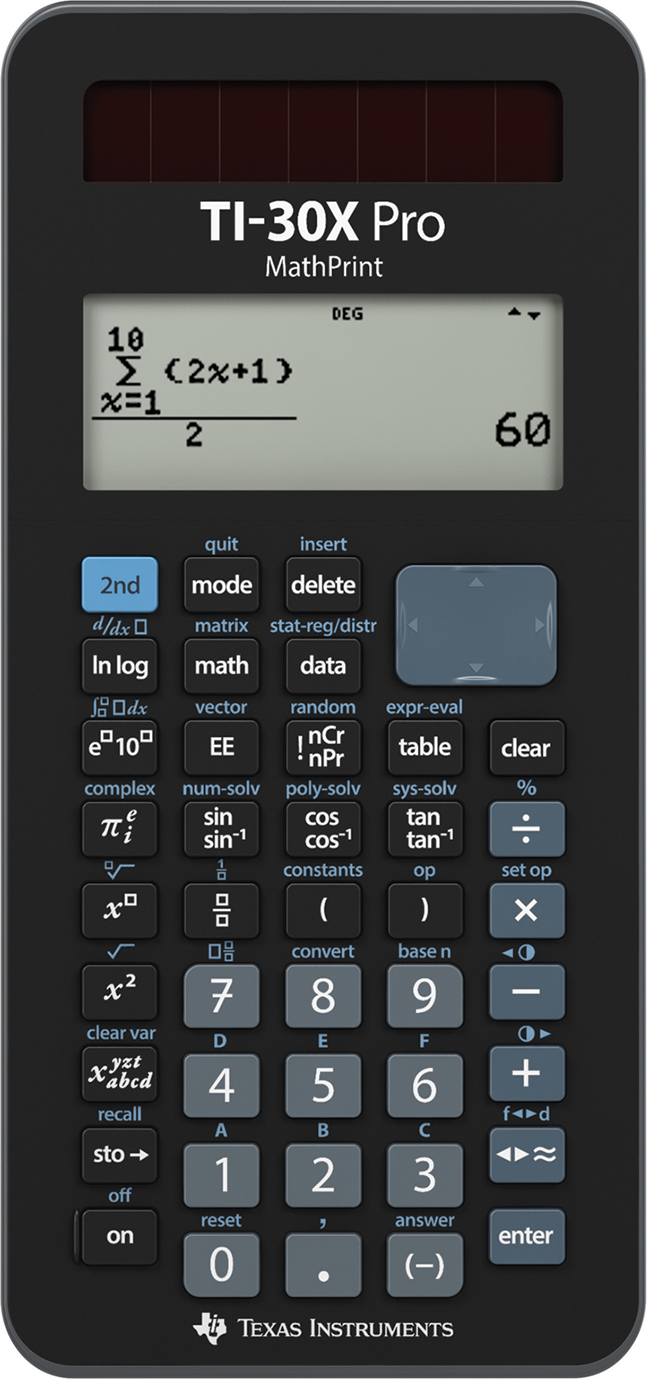
\includegraphics[width=45mm]{img/tiprobuttonimages/ti30.png}}
&

\begin{tabular}{c|c|p{80mm}}\hline
\tiprobutton{math}         &Summe             & Summenzeichen $\Sigma$ (\tiprobutton{5})\\
                           &Faktorzerlegung   & Faktorzerlegung (\tiprobutton{4}\texttt{Pfactor})\\
                           & ggT, kgV         & gcd = ggT
(\tiprobutton{3}), lcm = kgV (\tiprobutton{2})\\\hline
                           &                  & Bestimmung statistischer Werte:\\
\tiprobutton{data}         & data             & Daten eingeben\\
                           &\texttt{stat-reg} & 1-VAR STATS anwählen
und \texttt{calc} drücken für Standardabweichung, Q1, Q3, Median, Min,
Max, Mittelwert etc.\\
                           &\texttt{distr}    & Bernoulliformel $\rightarrow$ 4: Binomial\textbf{p}df\\
                           &                  & Kumuliert $\rightarrow$ 5: Binomial\textbf{c}df\\\hline
\tiprobutton{cos_poly-solv}&\texttt{poly-solv}&  Quadratische Gleichungen in Grundform $ax^2+bx+c=0$\\
                           &                  &  (Auch für Zweiklammeransatz)\\\hline
\tiprobutton{tan_sys-solv} &\texttt{sys-solv} &  Lineare Gleichungssysteme\\\hline
\tiprobutton{sin_num-solv} &\texttt{num-solv} &  Gleichungen ($7^x=3^{2x+1}$) mit Zahlen nach $x$ auf\/lösen (hier $x\approx{}-4.37$).\\\hline
\tiprobutton{table}        & table            &  Wertetabelle für diverse Funktionen: Lineare Fkt., Potenzfkt., Exponentialfkt.\\\hline
\tiprobutton{ncrnpr}       &Kombinatorik      &  Fakultät: {\color{red}\textbf{!}}\\
                           &                  &  Kombination $n \choose k$ tippe $n$ nCr $k$\\
                           &                  &  Permutation $\frac{n!}{(n-k)!}$ tippe $n$ nPr $k$\\\hline
\tiprobutton{ln_log}       &  Logarithmen     &  log = Zehnerlogarithmus ($\lg$)\\
                           &                  &  ln  = Log. zur Basis $e$\\
                           &                  &  3x drücken = log zu beliebiger Basis\\\hline
\tiprobutton{sto_recall}   & Werte speichern  &  Erst \texttt{sto} drücken, danach können die Variablen gespeichert werden (\tiprobutton{xyzabcd}). \\\hline
\tiprobutton{xyzabcd}      &                  & Benutzen und Auslesen der Variablen.\\\hline
\tiprobutton{approx}       & Resultat-Anzeige  & $\sqrt{50}$ = $5\sqrt{2} \approx 7.0711$
\end{tabular}
\end{tabular}

\TRAINER{Generelle Fragen:\\
Fehlen Lernziele? Sind Lernziele zu viel?\\
Sind Beispiele zu viel/zu wenig?\\
Hat es genügend Platz für die SuS (Schülerinnen und Schüler) für weitere Notizen/Beispiele/Rezepte/Vorgehen?\\
Ganz am Schluss:

* Rechtschreibeprogramm
* Zeilenumbrüche und Einzüge (0pt bei Aufzählungen und Nummerierungen)
\keinHeaderUndKeinFooter{}

* Absatz-Umbrüche / Seitenumbrüche
}
\keinHeaderUndKeinFooter{}

%
\noTRAINER{\vspace{15mm}}%
%
%%\noTRAINER{\mmPapier{4}}%
%
\keinHeaderUndKeinFooter{}
\newpage
\keinHeaderUndKeinFooter{}

%%%%%%%%%%%%%%%%%%%%%%%%%%%%%%%%%%%%%%%%%%%%%%
%%           Notizen                        %%
%%%%%%%%%%%%%%%%%%%%%%%%%%%%%%%%%%%%%%%%%%%%%%

Eigene Notizen\\

\noTRAINER{\mmPapier{22}}%
\TRAINER{\mmPapier{20}}%
%
\vspace{5mm}

Fehler gefunden? \texttt{philipp.freimann@bbw.ch / christian.hersberger@bbw.ch}
%%v 0.0.29 DRAFT 2021-06-22 fp)}

\TRAINER{
{\footnotesize Quelltext dieser Formelsammlung:\\
\texttt{https://github.com/pheek/bbwMathe/tree/main/arbeitsblaetter/formelsammlung}}

{\footnotesize Version \versionsnummerFoSa{}}
}%% END TRAINER


\end{document}
